\documentclass[a4paper]{article}

% CJK support: prefer ctex, fallback to XeTeX native line breaking
\IfFileExists{ctex.sty}{
  \usepackage[fontset=fandol]{ctex}
}{
  % Fallback for minimal TeX installs (e.g. MacTeX Basic, TeX Live scheme-basic)
  % without ctex/xeCJK. Uses XeTeX's built-in CJK line breaking.
  \usepackage{fontspec}
  \XeTeXlinebreaklocale "zh"
  \XeTeXlinebreakskip = 0pt plus 1pt
  \IfFontExistsTF{Songti SC}{\setmainfont{Songti SC}}{%
    \IfFontExistsTF{Noto Serif CJK SC}{\setmainfont{Noto Serif CJK SC}}{}%
  }
  \IfFontExistsTF{Heiti SC}{\setsansfont{Heiti SC}}{%
    \IfFontExistsTF{Noto Sans CJK SC}{\setsansfont{Noto Sans CJK SC}}{}%
  }
}

% Basic packages
\usepackage{amsmath, amssymb}
\usepackage{graphicx}
\usepackage[margin=2.5cm]{geometry}
\emergencystretch=3em
\usepackage[most]{tcolorbox}
\usepackage{etoolbox}
\usepackage{listings}
\usepackage{hyperref}
\usepackage{booktabs}
\usepackage{array}
\usepackage{subcaption}
\usepackage{float}
\usepackage{tikz}
\IfFileExists{pgfplots.sty}{
    \usepackage{pgfplots}
    \pgfplotsset{compat=1.18}
}{}

% ===== Highlight boxes =====
\newtcolorbox{knowledgebox}[1]{
    enhanced, colback=blue!5!white, colframe=blue!75!black, colbacktitle=blue!75!black,
    coltitle=white, fonttitle=\bfseries, title={#1}, attach boxed title to top left={yshift=-2mm, xshift=2mm},
    boxrule=1pt, sharp corners
}

\newtcolorbox{importantbox}[1]{
    enhanced, colback=yellow!10!white, colframe=yellow!80!black, colbacktitle=yellow!80!black,
    coltitle=black, fonttitle=\bfseries, title={#1}, sharp corners
}

\newtcolorbox{warningbox}[1]{
    enhanced, colback=red!5!white, colframe=red!75!black, colbacktitle=red!75!black,
    coltitle=white, fonttitle=\bfseries, title={#1}, sharp corners
}

\newtcolorbox{practicebox}[1]{
    enhanced, colback=black!3!white, colframe=black!75, colbacktitle=black!75,
    coltitle=white, fonttitle=\bfseries, title={#1}, sharp corners
}

% ===== Code listings =====
\lstset{
    basicstyle=\ttfamily\small,
    keywordstyle=\color{blue},
    stringstyle=\color{red!60!black},
    commentstyle=\color{green!60!black},
    breaklines=true,
    frame=single,
    numbers=left,
    numberstyle=\tiny\color{gray},
    captionpos=b,
    extendedchars=false
}

% ===== Figure provenance and unit macros =====
% \vtag goes inside \caption{...}; \srcnote{MM:SS--MM:SS} follows the figure environment.
\newcommand{\vtag}{\protect\footnotemark}
\newcommand{\srcnote}[1]{\footnotetext{视频画面时间区间：#1。若为裁剪图，时间区间仍对应原视频画面。}}
% Units work in text and math mode; never hand-write $^\circ$ or \AA inside \mathrm.
\newcommand{\degC}{\ensuremath{^{\circ}\mathrm{C}}}
\newcommand{\um}{\ensuremath{\mu\mathrm{m}}}
\newcommand{\nm}{\ensuremath{\mathrm{nm}}}
\newcommand{\angstrom}{\ensuremath{\text{\AA}}}

% ===== Front-page metadata =====
% Fill these in when generating notes.
\newcommand{\notetitle}{开发环境与工具}
\newcommand{\notesubtitle}{MIT Missing Semester 2026 · 第 3 讲：Vim 编辑语言、语言服务器与 AI 辅助编程}
\newcommand{\noteauthors}{根据 MIT Missing Semester 2026 课堂录像整理（Anish 主讲）}
\newcommand{\notedate}{2026年1月14日（课堂）}
\newcommand{\videochannel}{Missing Semester（YouTube）}
\newcommand{\videopublishdate}{2026年}
\newcommand{\videoduration}{53分48秒}
\newcommand{\videourl}{https://www.youtube.com/watch?v=QnM1nVzrkx8}
\newcommand{\videocoverpath}{cover.jpg}

\setlength{\emergencystretch}{3em}
\begin{document}

% ===== Title page =====
\begin{titlepage}
\centering
{\Large 课程笔记\par}
\vspace{1.2cm}
{\huge\bfseries \notetitle\par}
\ifdefempty{\notesubtitle}{}{
\vspace{0.3cm}
{\large \notesubtitle\par}
}
\vspace{0.5cm}
{\large \noteauthors\par}
\vspace{0.3cm}
{\large \notedate\par}
\vspace{1.0cm}

\ifdefempty{\videocoverpath}{
{\small 请在生成笔记时填入视频封面图的本地路径。\par}
}{
\includegraphics[width=0.82\textwidth,height=0.40\textheight,keepaspectratio]{\videocoverpath}\par
}

\vfill
\begin{tcolorbox}[width=0.9\textwidth, colback=black!2!white, colframe=black!60, sharp corners]
\textbf{视频作者/频道}：\videochannel\par
\textbf{发布日期}：\videopublishdate\par
\textbf{视频时长}：\videoduration\par
\textbf{视频链接}：
\ifdefempty{\videourl}{
未填写
}{
\href{\videourl}{\nolinkurl{\videourl}}
}
\end{tcolorbox}
\end{titlepage}

\tableofcontents
\newpage

%% --- 正文内容开始 --- %%

\section{这一讲讲什么}

这是 Missing Semester 第三天的课，主题是开发环境与工具。讲者 Anish 一开始就说，这一讲计划塞进非常多的子主题，所以希望课堂尽量互动：多提问，也帮他把握节奏，告诉他是该多讲基础，还是快速带过基础、把时间留给更进阶的内容。

\noindent\begin{minipage}{\textwidth}
\begin{figure}[H]
\centering
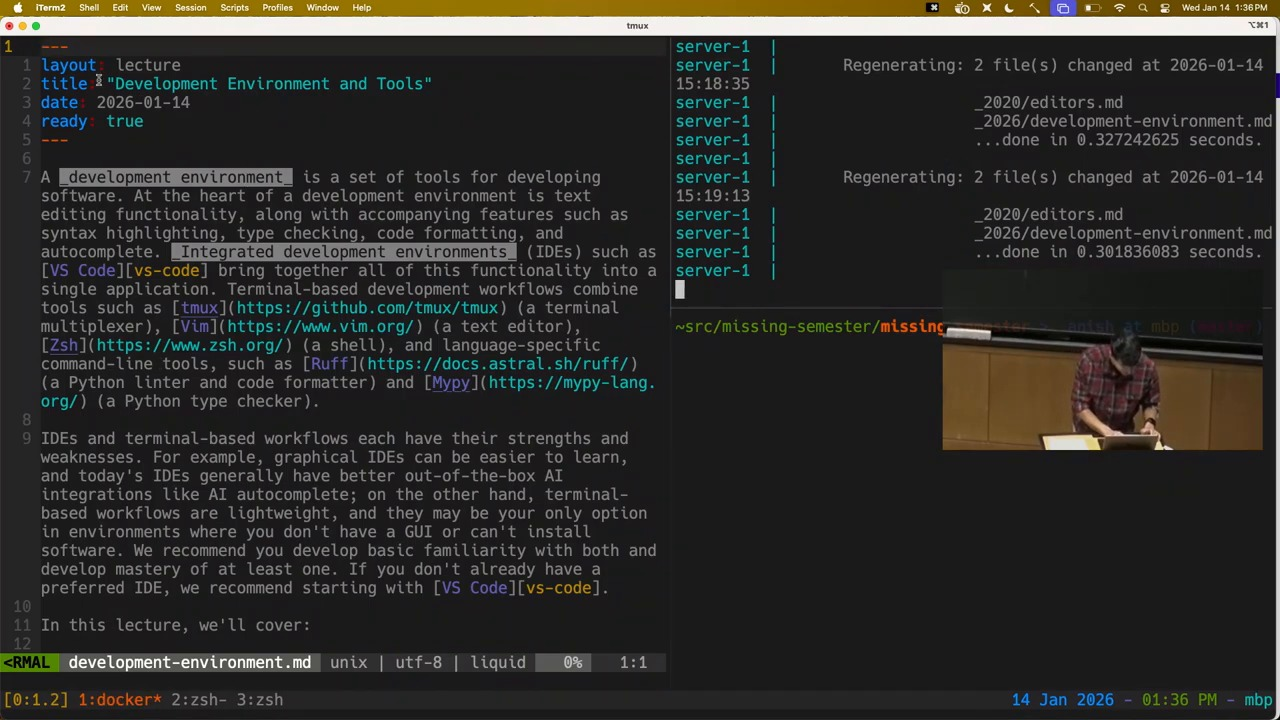
\includegraphics[width=0.92\textwidth]{figures/fig_01_tmux_setup.jpg}
\caption{讲者的终端开发环境：tmux 分屏，右下角用 Vim 打开今天的讲义\vtag}
\end{figure}
\srcnote{00:01:00--00:01:15}
\end{minipage}


什么是开发环境？就是一套开发软件用的工具，形式多种多样。屏幕上是讲者的终端环境：他用上一讲介绍过的 tmux 分割窗格，右下角的 Shell 里用 Vim 打开了今天的讲义，右上角的终端里运行着 Docker。这是一种基于终端的开发环境，适合某些场景。

\noindent\begin{minipage}{\textwidth}
\begin{figure}[H]
\centering
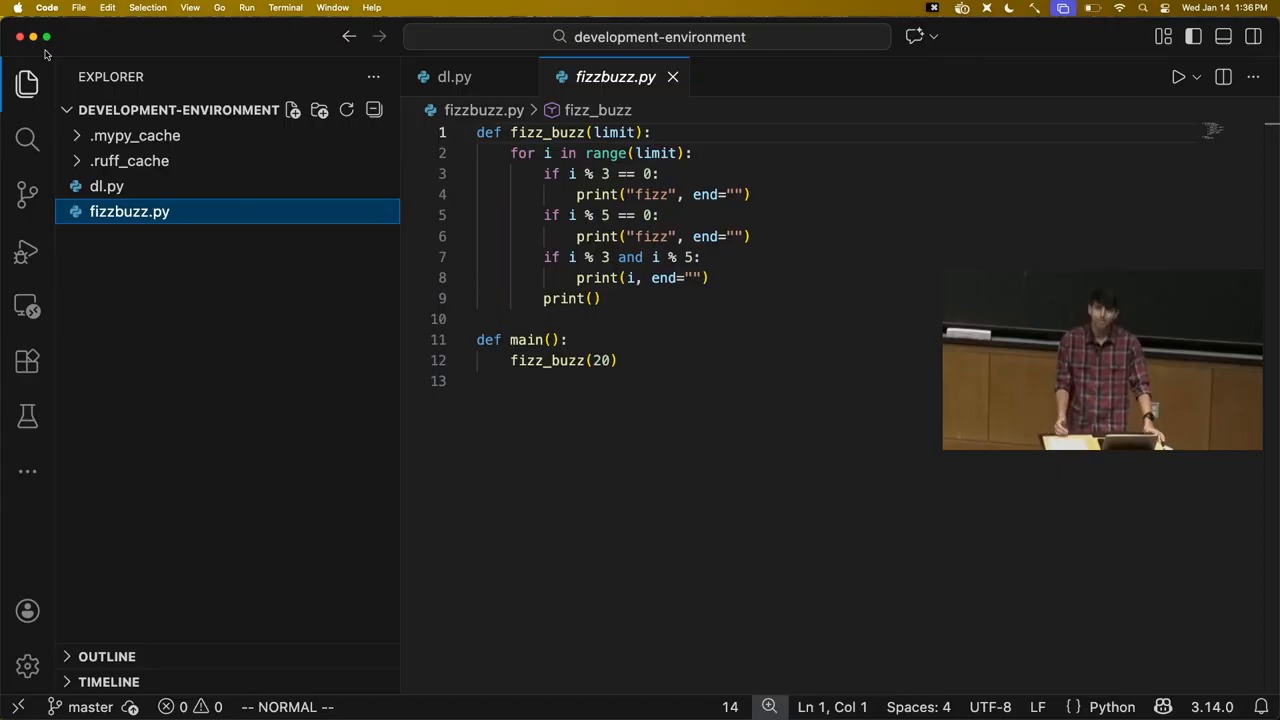
\includegraphics[width=0.92\textwidth]{figures/fig_02_vscode.jpg}
\caption{另一种形态：把编辑、检查、格式化集成在一起的 VS Code\vtag}
\end{figure}
\srcnote{00:01:15--00:01:30}
\end{minipage}


在另一些场景下，你可能想用 VS Code 这样的集成开发环境（IDE）。它和终端方案不太一样：从文本编辑到代码检查（linting）、自动格式化等你可能需要的一切，都集中在一个应用里。讲者说，当把这些东西放在一处有好处时，就适合用图形化 IDE；而且 AI 功能往往和图形化 IDE 集成得更好，所以它是不错的起点。但在某些情况下也值得学会基于终端的开发，比如你 SSH 到一台远程机器上，没法方便地安装软件时。

有同学问 IDE 和文本编辑器的区别。讲者解释，IDE 即集成开发环境，就是把一切放在一处；也有运行在终端里的文本界面 IDE。Emacs、Vim 这类程序本身更像文本编辑器，但可以装一堆插件，让它们表现得更像 IDE，所以他才这样区分；不过粗略地说，人们说 IDE 时一般指图形化 IDE。屏幕上这个是 VS Code，微软的一个非常流行的开源 IDE。讲者问有多少人听说过 Cursor，相当一部分人举了手；他补充说 Cursor 是 VS Code 的一个分支（fork），构建在它之上。

\begin{knowledgebox}{本讲计划的内容}
讲者列出的计划是：先讲用 Vim 编辑文本，因为文本编辑是 IDE 的核心功能；然后讲代码智能与语言服务器，也就是代码补全、边写边检查错误等更进阶的 IDE 功能；接着是这一轮课程新增的 AI 辅助开发；最后简要讲正则表达式与查找替换。讲义作者注：实际课上时间不够，AI 部分只讲到自动补全和行内聊天，编码智能体和正则表达式被推迟到后面的课程。
\end{knowledgebox}

\section{为什么学 Vim}

\subsection{编辑代码不同于写文章}

讲者问有多少人用过或听说过 Vim，大约四分之一的人举手。他说，前几讲已经有不少地方提到 Vim，这一讲就是专门讲它的，配套也有一批 Vim 相关的习题。

他解释为什么想教 Vim：写代码时，你面对一堆文本并修改它，但交互和修改的方式与其他类型的文本编辑不同。写论文时你可能用 Word，主要是从头到尾写一长串文字，或者从上到下读一长串文字。编辑代码却不一样：你经常在文件之间跳来跳去，读一小段一小段的代码。即使是写代码，你有多少次是打开一个新文件，从头到尾一口气写完整个程序？讲者问谁有这么厉害，没有人举手。所以你常常是写一小段：这里写个函数，跳到文件上面写另一个函数，在某处发现 bug 再调整代码。光标需要的移动方式、需要输入的文本类型都不同。

\subsection{核心思想：界面就是一门编程语言}

讲者说，Vim 既是文本编辑器，也是一种为这种用途优化过的、与文本缓冲区交互的方式；学会它，就能在写软件时非常高效地编辑文本。开发 Vim 及其前身 vi 的人观察到，在键盘和鼠标之间切换很慢：想把光标从下面移到上面，要把手从键盘移到鼠标，移动指针，点击，然后才能开始打字。如果手指能一直放在键盘上，并且有一个非常高效的界面完成编辑代码时的各种操作，就会快得多。

所以 Vim 的核心思想是：Vim 的界面本身可以看作一门编程语言。就像编程语言一样，它有一组基本元素（primitives），可以组合起来做强大的事。

\noindent\begin{minipage}{\textwidth}
\begin{figure}[H]
\centering
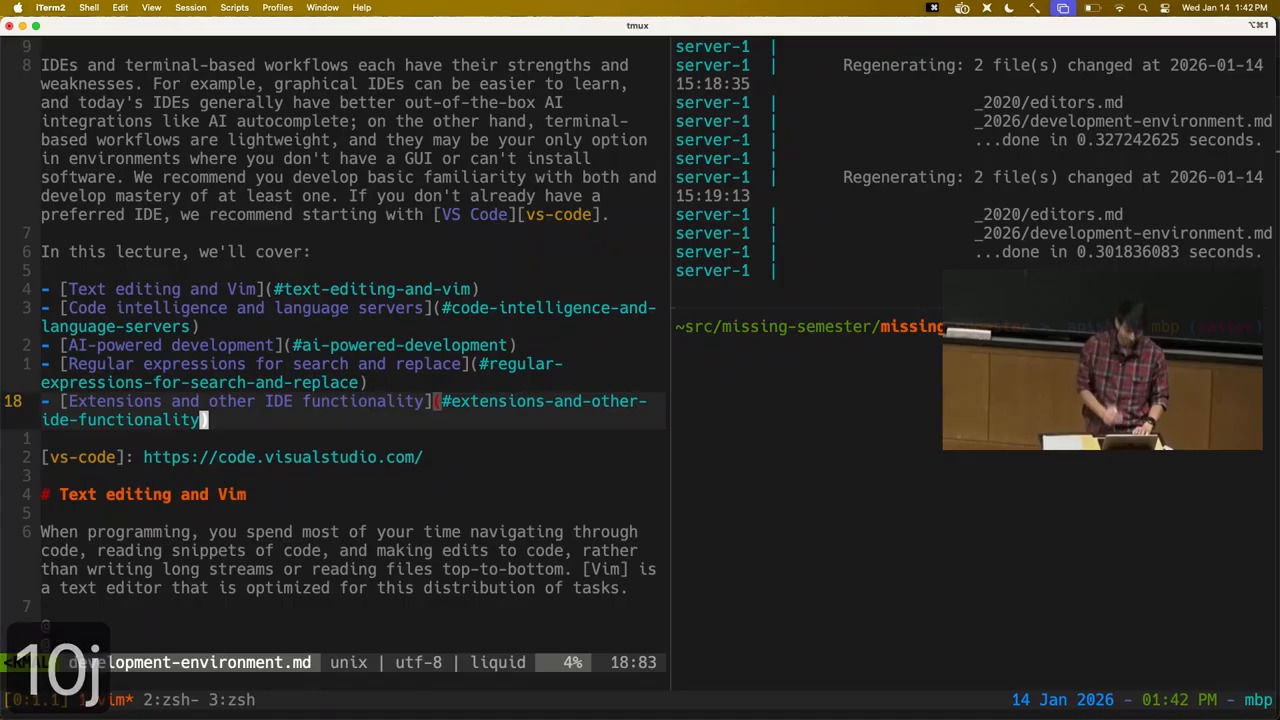
\includegraphics[width=0.92\textwidth]{figures/fig_03_keycaster.jpg}
\caption{按键显示工具在右下角显示 10j：一次向下跳 10 行\vtag}
\end{figure}
\srcnote{00:07:00--00:07:15}
\end{minipage}


讲者打开了一个按键显示工具，屏幕下方会显示他按下的键。比如 \texttt{j} 键让光标下移一行；想下移 10 行，就输入 \texttt{10j}，一次跳下 10 行。想找下一个某字符，按 \texttt{f} 加字符，光标就跳过去；按 \texttt{\%} 跳到匹配的括号；想修改后面括号里的内容，用 \texttt{ci(}，括号里的内容被删除，然后就可以输入新内容。讲者说，这看起来和你习惯的其他 IDE 很不一样：通常你会移动鼠标，点到这里，再按退格把里面的东西都删掉，或者点击拖动选中再按退格；而用 Vim 作为与文本缓冲区交互的方式要快得多。

\section{模式编辑}

\subsection{Vim 的几种模式}

\noindent\begin{minipage}{\textwidth}
\begin{figure}[H]
\centering
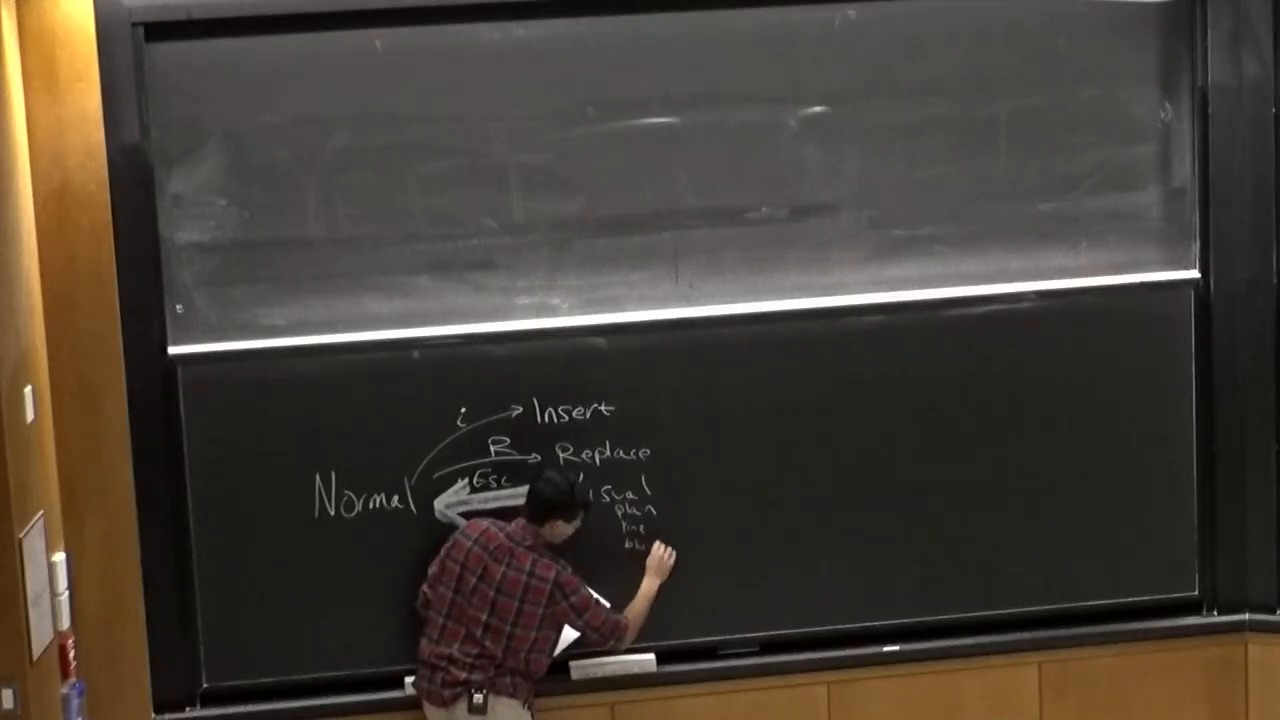
\includegraphics[width=0.92\textwidth]{figures/fig_04_modes_board.jpg}
\caption{黑板上的模式图：普通模式居中，通过不同的键进入插入、替换、可视和命令模式\vtag}
\end{figure}
\srcnote{00:09:30--00:09:45}
\end{minipage}


讲者说，Vim 是所谓的模式编辑器（modal editor）：有不同的操作模式，分别用来做不同类别的事情。
\begin{itemize}
\item 普通模式（normal mode）：默认模式，启动时就在这里，你会在这里度过大部分时间；
\item 插入模式（insert mode）：用来插入和添加文本，从普通模式按 \texttt{i} 进入，按 Esc 回到普通模式。在插入模式下，Vim 和你用过的任何文本编辑器一样，按下的键直接输入到文本缓冲区；
\item 替换模式（replace mode）：按大写 \texttt{R} 进入，用来覆盖已有的文本；
\item 可视模式（visual modes）：普通可视模式按 \texttt{v}，可视行模式按大写 \texttt{V}，可视块模式按 Ctrl+V，分别用来选择一段文本、若干行或一个矩形块；
\item 命令模式（command mode）：按冒号进入，用来运行命令。
\end{itemize}

讲者提到，Vim 的键位命名得很方便记忆，比如 \texttt{i} 就是 insert。

\noindent\begin{minipage}{\textwidth}
\begin{figure}[H]
\centering
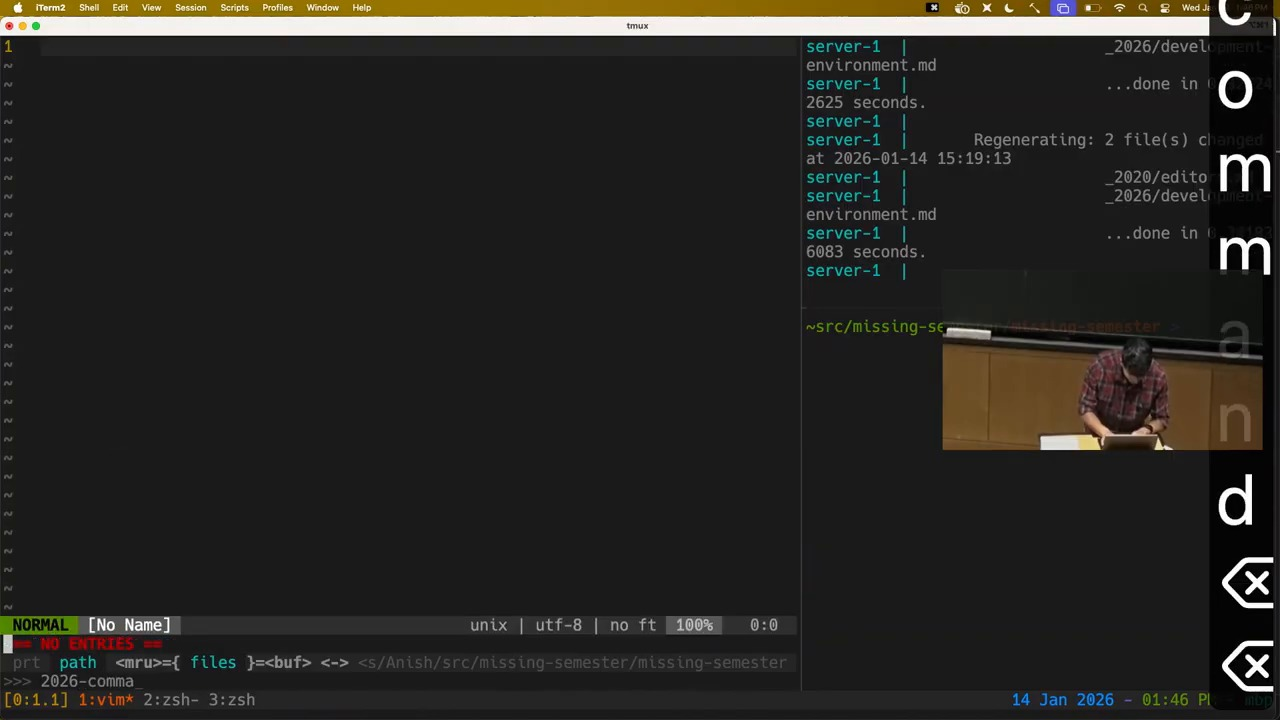
\includegraphics[width=0.92\textwidth]{figures/fig_05_quit.jpg}
\caption{按冒号进入命令模式，底部出现命令行，输入 q 退出\vtag}
\end{figure}
\srcnote{00:11:00--00:11:15}
\end{minipage}


有同学问“关闭”是不是一个命令。讲者说是的，在 Vim 里关闭就是一个命令。他的 Vim 设置成在左下角显示当前模式；按冒号进入命令模式后，底部出现命令行，输入 \texttt{q} 再回车。因为有未保存的修改，Vim 拒绝退出；他用 \texttt{q!} 强制退出了编辑器。

\subsection{Vim 的思想无处不在}

讲者强调，即使你不用 Vim 这个软件本身，Vim 的思想也强大到许多其他软件都支持 Vim 键位：VS Code 这样的 IDE、另一个命令行文本编辑器 Emacs，前两讲讲过的 zsh 和 bash，甚至 Claude Code，都支持 Vim 模式的键位。所以学会这种与文本缓冲区交互的方式，就能把它用在许多不同的程序里。

上一轮课程专门讲的是 Vim 这个软件；这一轮关注的是 Vim 的核心思想，以及 Vim、Neovim 和 VS Code 的 Vim 实现之间共通的键位，以便把这些思想带到任何地方。所以像怎样退出 Vim、\texttt{:wq} 之类的内容，今年不是重点，因为如果你用 VS Code，想关掉什么点叉号就行。

\begin{importantbox}{学习重点：可迁移的键位语言}
今年的课程不追求掌握 Vim 软件的全部配置，而是学会那套在各种编辑器、Shell 和工具里通用的键位语言。在你常用的软件里打开 Vim 模式，收益就会出现在所有地方。
\end{importantbox}

\subsection{从插入模式起步}

\noindent\begin{minipage}{\textwidth}
\begin{figure}[H]
\centering
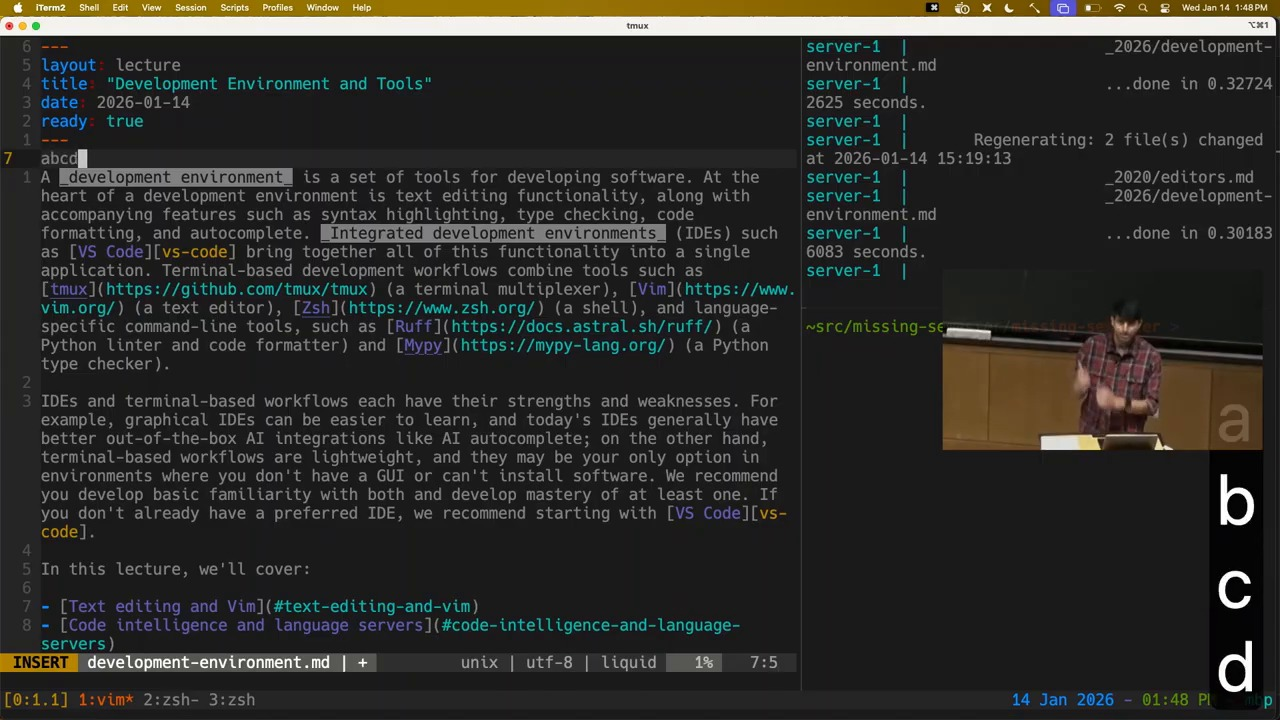
\includegraphics[width=0.92\textwidth]{figures/fig_06_insert.jpg}
\caption{按 i 进入插入模式后，输入的 abcd 直接进入缓冲区\vtag}
\end{figure}
\srcnote{00:13:00--00:13:15}
\end{minipage}


讲者建议，刚开始用 Vim 时，在使用那些复杂功能之前，可以先只靠普通模式和插入模式，把它当作普通的文本编辑器。在普通模式下不能直接修改内容，按 \texttt{i} 进入插入模式，输入比如 abcd，文本就插入到缓冲区里，表现和其他编辑器一样，可以用方向键移动，配置得当的 Vim 或者 VS Code 里还可以用鼠标。但这样使用 Vim 就没有利用它的强大功能。真正要做的是利用 Vim 界面作为一门编程语言的特点，高效地移动和编辑，为此要更多地使用插入模式以外的模式，特别是普通模式。

\section{普通模式：一门编辑语言}

\noindent\begin{minipage}{\textwidth}
\begin{figure}[H]
\centering
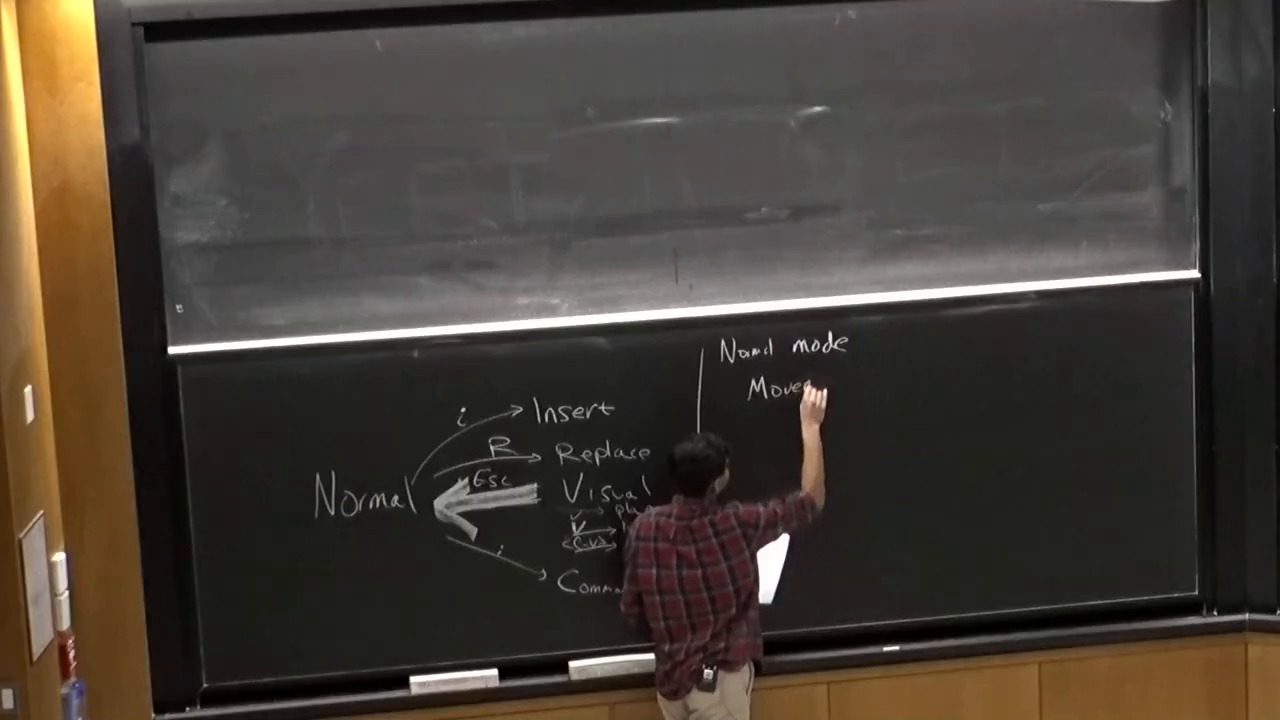
\includegraphics[width=0.92\textwidth]{figures/fig_07_grammar_board.jpg}
\caption{黑板上的普通模式组成：移动、选择、编辑、计数与修饰符\vtag}
\end{figure}
\srcnote{00:14:00--00:14:15}
\end{minipage}


讲者在黑板上写出普通模式中的几类键位：移动、选择、编辑，还有计数，以及额外的修饰符。它们可以以强大的方式组合在一起。他再三强调现在不用记这些具体键位：讲义里链接了很多资源，可以帮助你真正记住它们；要关注的是怎样把它们组合起来、非常高效地完成编辑，而不是像基线方法那样把手从键盘挪到鼠标上、移动指针、到处点击。

\subsection{移动}

\noindent\begin{minipage}{\textwidth}
\begin{figure}[H]
\centering
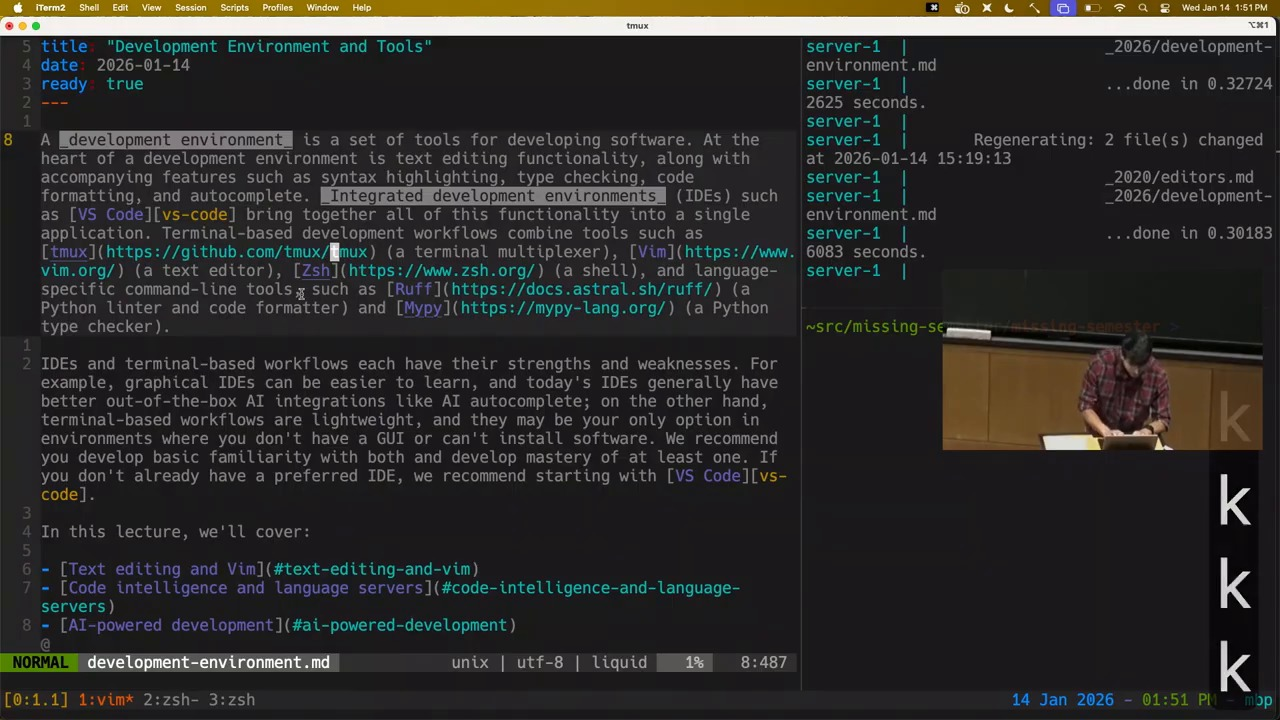
\includegraphics[width=0.92\textwidth]{figures/fig_08_movement.jpg}
\caption{在普通模式下用 hjkl、w、b 等键移动光标\vtag}
\end{figure}
\srcnote{00:15:30--00:15:45}
\end{minipage}


基本移动：上下左右可以用方向键；Vim 还把 \texttt{h}、\texttt{j}、\texttt{k}、\texttt{l} 绑定到四个方向，这样手不必离开主键位行，节省那一点点时间。按 \texttt{h} 光标左移，\texttt{l} 右移，\texttt{j} 下移一行，\texttt{k} 上移一行。还有很多键位：
\begin{itemize}
\item \texttt{w} 每次向前移动一个单词，\texttt{b} 回到单词开头，它们都是助记的，w 表示 word，b 表示 back 或 beginning；
\item \texttt{0} 到行首，\texttt{\$} 到行尾；
\item \texttt{H}、\texttt{M}、大写 \texttt{L} 分别到屏幕顶部、中部和底部；
\item Ctrl+D 向下滚动，Ctrl+U 向上滚动；
\item \texttt{gg} 到文件第一行，大写 \texttt{G} 到最后一行；
\item 输入冒号加行号（比如 \texttt{:123}）再回车，跳到那一行；
\item \texttt{\%} 在匹配的括号之间跳转；
\item \texttt{f} 加一个字符，跳到下一个该字符，例如 \texttt{fb} 找到下一个 b，\texttt{fw} 找到下一个 w；\texttt{t} 类似，但停在字符之前。
\end{itemize}

讲者说这里已经能看到组合：\texttt{f} 和后面的字符一起构成一个完整的移动。

\noindent\begin{minipage}{\textwidth}
\begin{figure}[H]
\centering
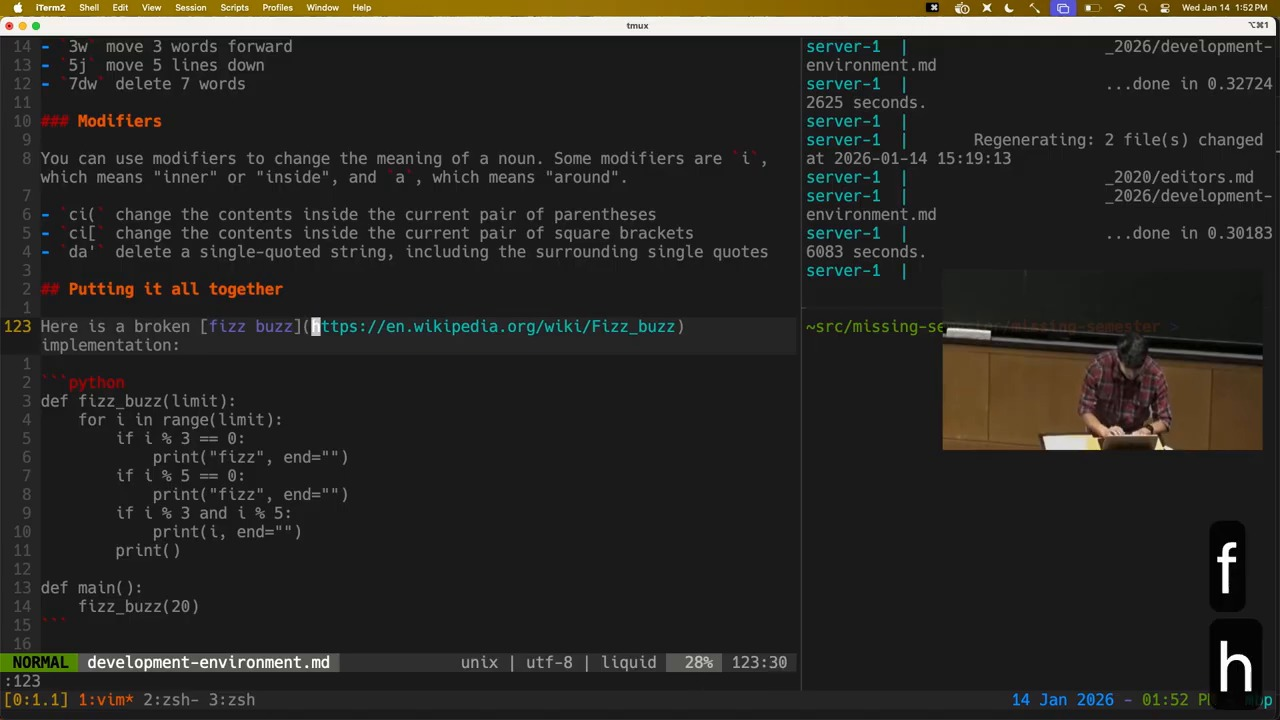
\includegraphics[width=0.92\textwidth]{figures/fig_09_search.jpg}
\caption{按斜杠输入 phys 搜索，光标跳到第一个匹配处\vtag}
\end{figure}
\srcnote{00:16:30--00:16:45}
\end{minipage}


另一个特殊的移动是搜索：按 \texttt{/}，输入比如 phys，回车，光标就跳到第一个匹配处。

\begin{knowledgebox}{移动命令速查}
讲义作者按课程讲义整理：\texttt{hjkl} 基本方向；\texttt{w}/\texttt{b}/\texttt{e} 下一个词首/词首/词尾；\texttt{0}/\texttt{\^{}}/\texttt{\$} 行首/首个非空字符/行尾；\texttt{H}/\texttt{M}/\texttt{L} 屏幕顶/中/底；\texttt{gg}/\texttt{G} 文件首/尾；\texttt{:\{行号\}} 跳到某行；\texttt{\%} 匹配括号；\texttt{f\{字符\}}/\texttt{t\{字符\}} 行内查找，用 \texttt{;} 和 \texttt{,} 在匹配之间前后移动；\texttt{/\{正则\}} 搜索，用 \texttt{n}/\texttt{N} 在匹配之间移动。
\end{knowledgebox}

\subsection{选择}

\noindent\begin{minipage}{\textwidth}
\begin{figure}[H]
\centering
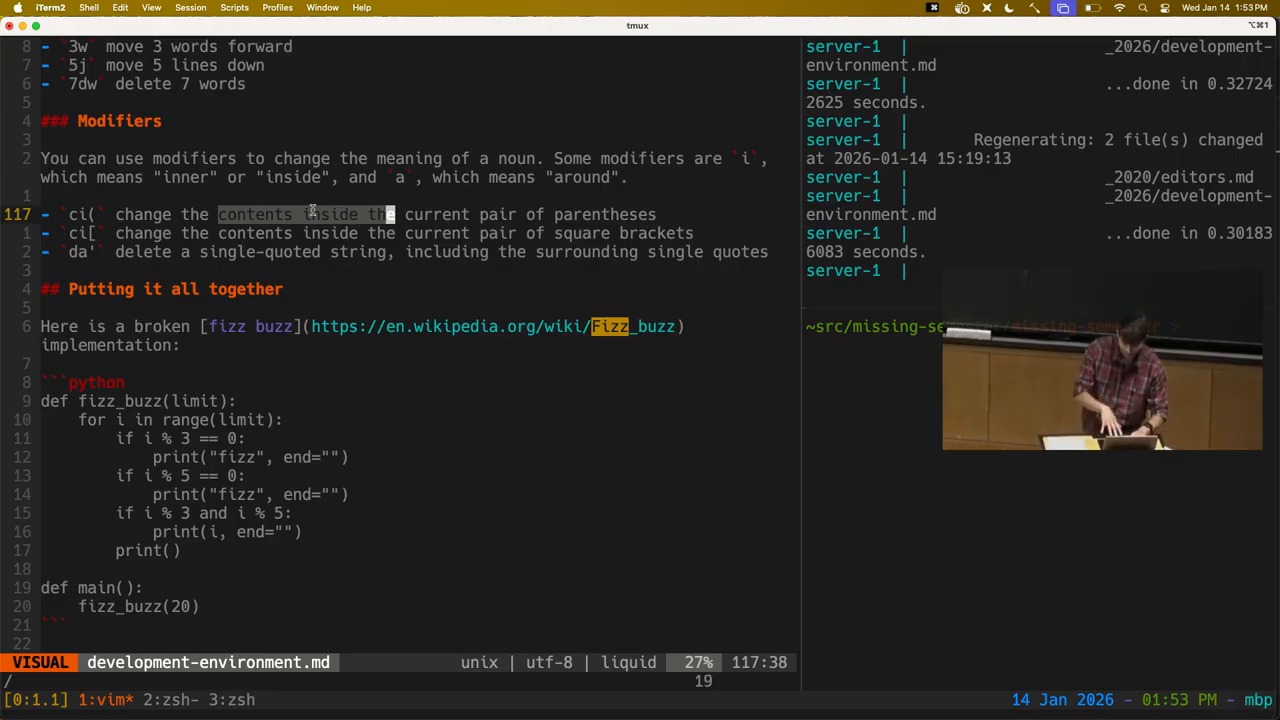
\includegraphics[width=0.92\textwidth]{figures/fig_10_visual.jpg}
\caption{按 v 进入可视模式，左下角显示 VISUAL，用移动键扩展选区\vtag}
\end{figure}
\srcnote{00:17:30--00:17:45}
\end{minipage}


选择用的是前面提到的可视模式。按 \texttt{v} 进入可视模式，左下角显示当前处于可视模式；再用移动命令移动光标，比如按 \texttt{w} 到下一个单词开头，就选中了这一段文本。大写 \texttt{V} 按行选择而不是按字符，按 \texttt{j} 就多选下一行。Ctrl+V 可以选择矩形块，这可能是你现在用的编辑器做不到的。

\subsection{编辑}

\noindent\begin{minipage}{\textwidth}
\begin{figure}[H]
\centering
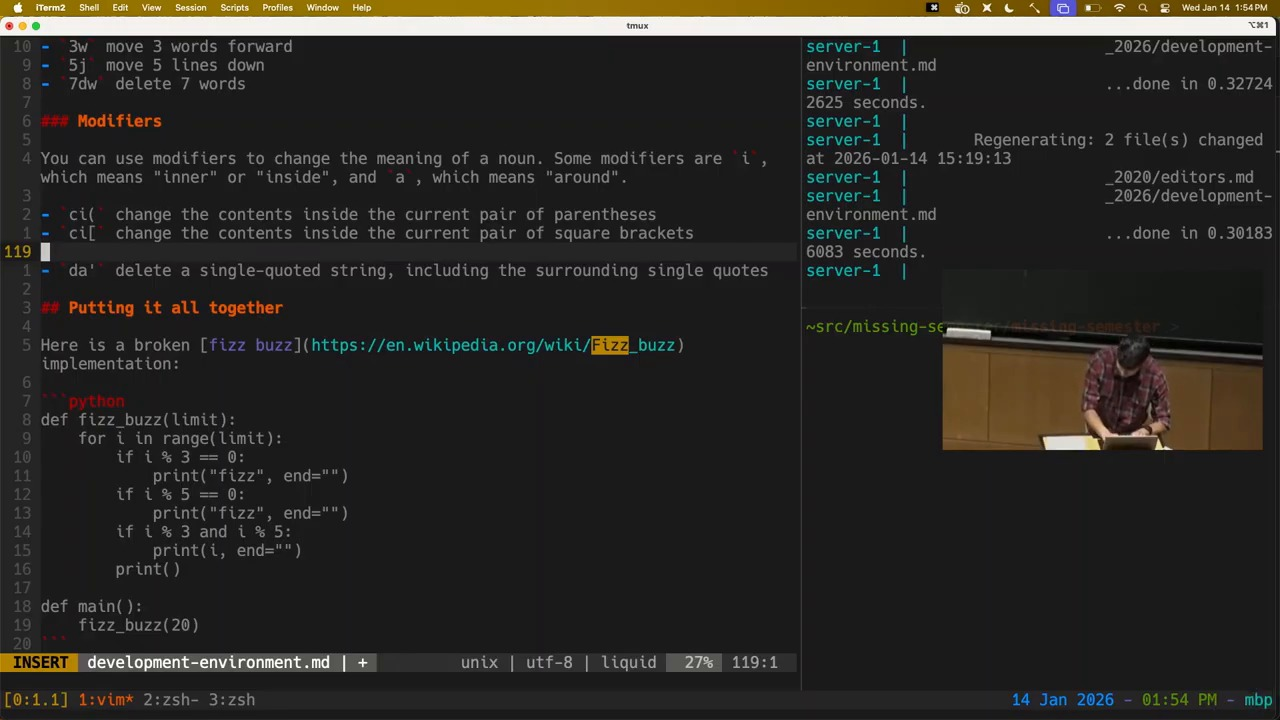
\includegraphics[width=0.92\textwidth]{figures/fig_11_edits.jpg}
\caption{o 在下方开一行并进入插入模式，d 与移动组合删除文本\vtag}
\end{figure}
\srcnote{00:18:30--00:18:45}
\end{minipage}


真正的编辑：插入模式让 Vim 回到直接输入的状态，此外还有许多做各种编辑的命令。比如在普通模式下按 \texttt{o}，在下方新建一行，这是对缓冲区的修改，同时进入插入模式；大写 \texttt{O} 在当前行上方新建一行并进入插入模式；\texttt{u} 撤销。

这些编辑命令可以和移动命令组合。比如光标在某处，想删除这个单词，可以按 \texttt{d} 表示删除，这个命令接受一个移动作为参数，\texttt{dw} 就删除一个单词；想删除这一行和下一行，用 \texttt{dj}：向下移动，并删除移动所覆盖的一切。

\begin{knowledgebox}{动词作用于名词}
课程讲义把编辑命令称为“动词”，因为动词作用于名词（移动或文本对象）：\texttt{d\{移动\}} 删除，例如 \texttt{dw}、\texttt{d\$}、\texttt{d0}；\texttt{c\{移动\}} 修改，相当于删除后进入插入模式，例如 \texttt{cw}；\texttt{x} 删除字符（等价于 \texttt{dl}），\texttt{s} 替换字符（等价于 \texttt{cl}）；可视模式选中后按 \texttt{d} 或 \texttt{c}；\texttt{u} 撤销，Ctrl+R 重做；\texttt{y} 复制（yank），\texttt{p} 粘贴；\texttt{\textasciitilde} 切换大小写，\texttt{J} 连接行。
\end{knowledgebox}

\subsection{计数}

讲者接着说计数。另一位讲者 Jon 在台下指出，计数不只适用于移动和编辑，而是适用于任何命令：在命令前加一个数字，就执行那么多次。比如把光标放在这里按 \texttt{5w}，就是执行五次 \texttt{w}，向前移动五个单词；也可以 \texttt{5u}，撤销五次。

\subsection{修饰符}

\noindent\begin{minipage}{\textwidth}
\begin{figure}[H]
\centering
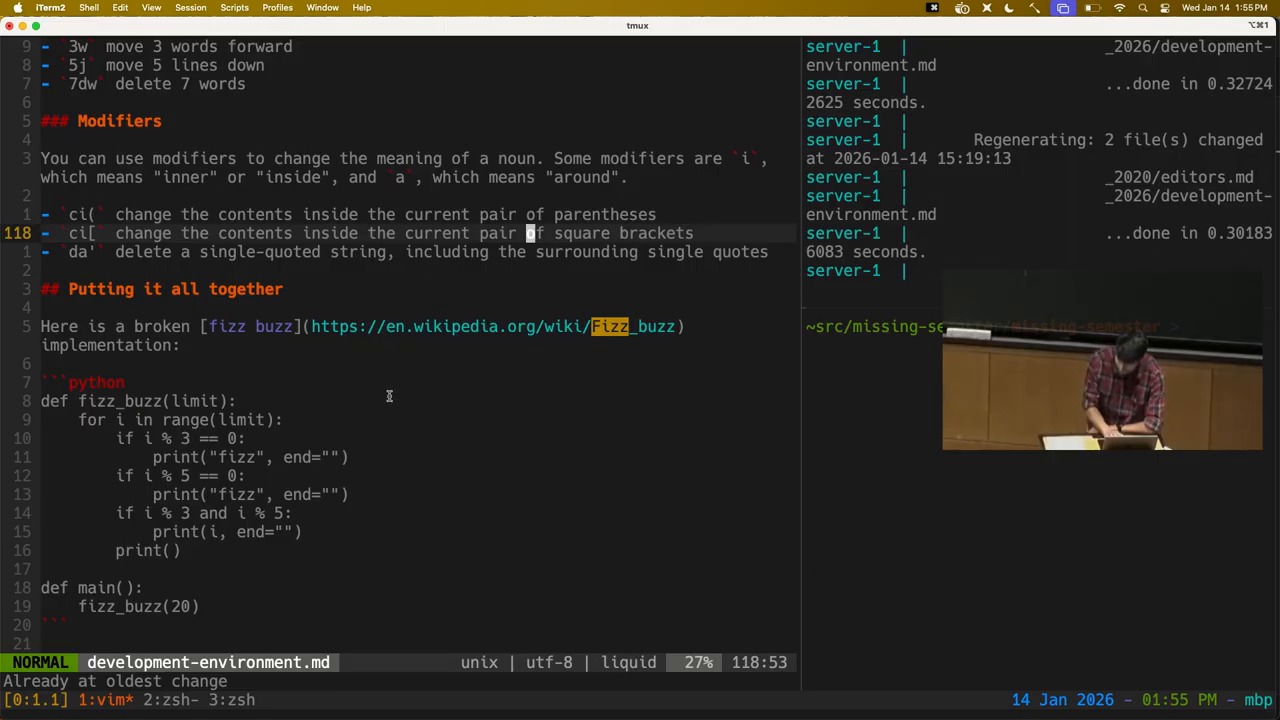
\includegraphics[width=0.92\textwidth]{figures/fig_12_ci_paren.jpg}
\caption{在 Markdown 链接的圆括号里按 ci( 删除链接地址并进入插入模式\vtag}
\end{figure}
\srcnote{00:20:00--00:20:15}
\end{minipage}


还有修饰符，用来改变某些名词的含义：\texttt{i} 表示 inside（内部），\texttt{a} 表示 around（周围）。比如光标在这里，这是 Markdown 里的一个链接，也许发现链接写错了，就可以按 \texttt{c} 表示修改，这是编辑命令；\texttt{i} 表示内部，这是修饰符；圆括号是名词，即要修改其内部内容的东西。讲者吐槽按键显示工具把左括号显示成了 Shift+9。\texttt{ci(} 删除当前所在圆括号内的内容并进入插入模式，就可以换成另一个链接。比如写代码时想修改函数的参数，\texttt{ci(} 就非常快。和标准 IDE 里的做法相比：把手从键盘挪到鼠标，移过去，点击拖动，按退格，再开始输入。

\begin{lstlisting}[language=bash]
ci(    change the contents inside the current pair of parentheses
ci[    change the contents inside the current pair of square brackets
da'    delete a single-quoted string, including the surrounding quotes
3w     move 3 words forward
7dw    delete 7 words
\end{lstlisting}

\subsection{怎样建立直觉}

讲者说他讲得很快，目的是让大家接触这些通用概念：移动、选择、编辑、计数、修饰符等不同类型的东西，学会之后就能组合起来，非常快地编辑。他说“你得相信我”：习题里建议把你用的所有软件都切换成 Vim 模式，强迫自己用一个月。他、Jon 和 Jose 三人都用 Vim 很久了，这份投入非常值得，基本可以达到“想多快就编辑多快”的程度；不用这样的界面，他觉得自己会把大量时间花在挪手上。他说这是一个好得多的“脑机接口”。

有同学问：撤销、重做、添加文本这类在别的编辑器里也有的功能，可以去找 Vim 里怎么做；但像跳到匹配括号、删除括号内部这类 Vim 特有的功能，怎么发现它们、建立直觉？讲者给出两点建议：一是做一份 Vim 教程，它会告诉你很多键位，并让你做文本编辑练习，把这些变成肌肉记忆；二是直接用 Vim，并时刻留意：如果你在做的事情显得重复又烦人，那么很可能有更好的办法，可以搜索、问 LLM，或者到课程的 Discord 发帖。他说这是程序员值得记住的好原则：最好的程序员里有一些非常“懒”的人；如果你花大量时间告诉电脑要怎样编辑文本，很可能已经有人想出了更好的办法并为你准备好了。

\begin{practicebox}{建立肌肉记忆}
讲义作者整理课程建议：先完成 \texttt{vimtutor}（终端里直接运行即可）；然后在 VS Code、Shell 等常用工具中开启 Vim 模式，坚持使用一个月；遇到重复操作时停下来查一查有没有更好的组合。不要试图一次记住所有键位，每周掌握几个新命令即可。
\end{practicebox}

\section{综合演示：修复 FizzBuzz}

\noindent\begin{minipage}{\textwidth}
\begin{figure}[H]
\centering
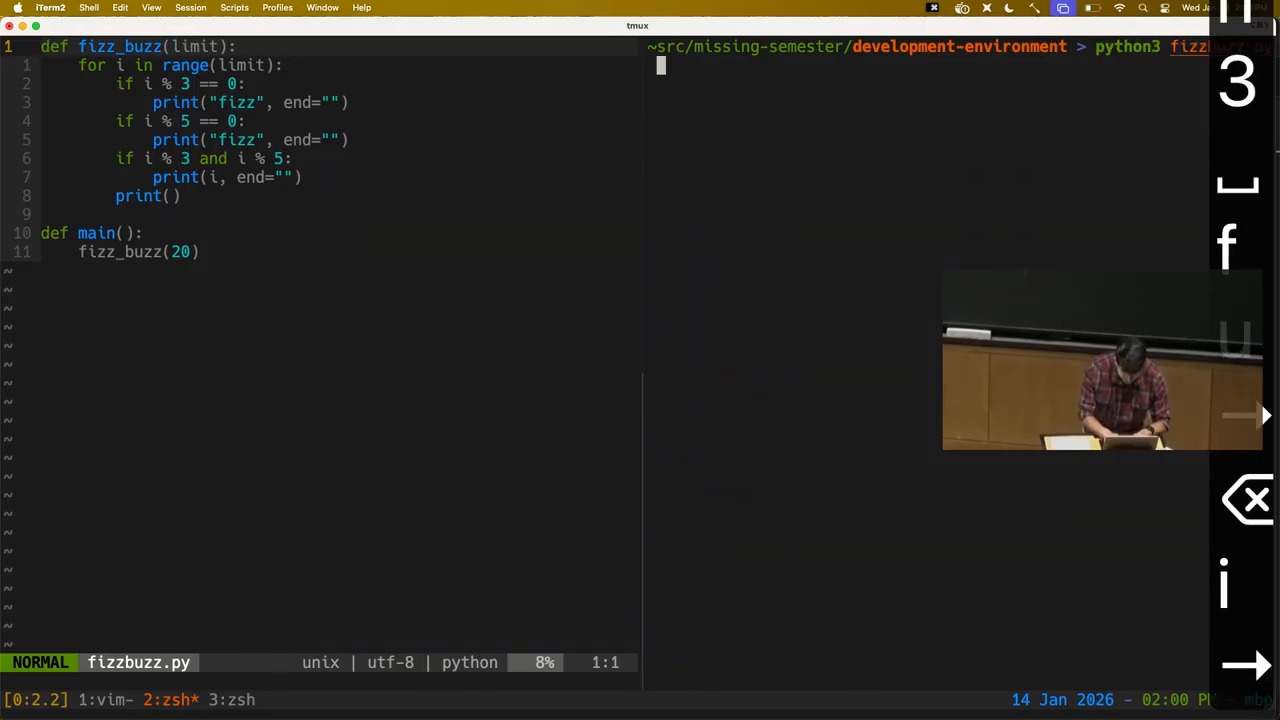
\includegraphics[width=0.92\textwidth]{figures/fig_13_fizzbuzz.jpg}
\caption{一个有问题的 FizzBuzz 实现，右侧终端运行它时没有任何输出\vtag}
\end{figure}
\srcnote{00:25:00--00:25:15}
\end{minipage}


讲者用修复一个有问题的 FizzBuzz 实现来演示怎样把这些部分组合起来。FizzBuzz 要求打印 1 到 $n$ 的数字，但遇到 3 的倍数时打印 fizz 代替数字，5 的倍数打印 buzz，同时是 3 和 5 的倍数时打印 fizzbuzz。讲者说这是检验会不会写代码的经典练习。屏幕上是一个有问题的实现，他要用 Vim 修好它，看看在按键次数上能有多高效。

\begin{lstlisting}[language=Python]
def fizz_buzz(limit):
    for i in range(limit):
        if i % 3 == 0:
            print("fizz", end="")
        if i % 5 == 0:
            print("fizz", end="")
        if i % 3 and i % 5:
            print(i, end="")
        print()

def main():
    fizz_buzz(20)
\end{lstlisting}

\subsection{第一处：main 从未被调用}

他在右边再开一个终端运行程序，什么都没发生，因为 \texttt{main} 函数从未被调用，这是第一处要修的。打开 Vim 时光标在顶部，而他想在底部添加文本：Vim 用一个键大写 \texttt{G} 就能跳到最后一行，按 \texttt{o} 开一个新行。他配了一些 Python 支持，所以编辑器自动缩进，以为他想继续写 \texttt{main} 的内容，他按退格删掉缩进，然后输入代码，按 Esc 回到普通模式。第一处修改完成。

\subsection{第二处：range 应从 1 开始}

\noindent\begin{minipage}{\textwidth}
\begin{figure}[H]
\centering
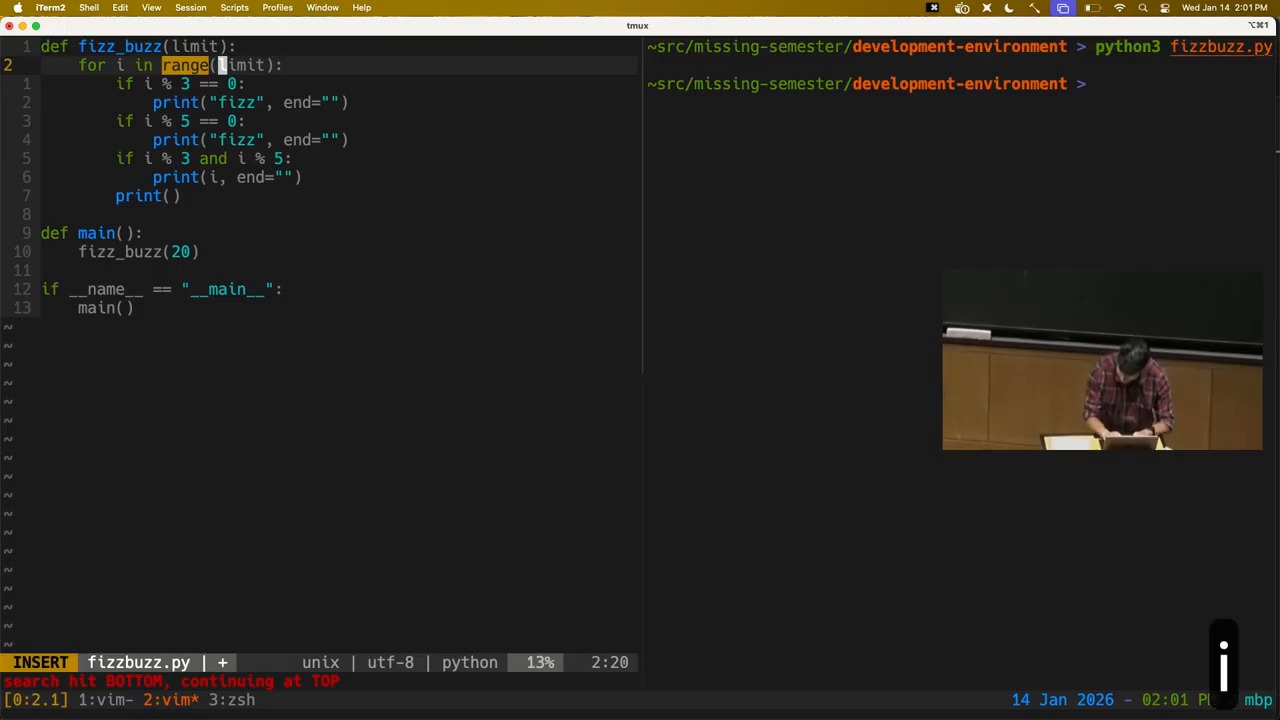
\includegraphics[width=0.92\textwidth]{figures/fig_14_fizz_range.jpg}
\caption{用 /range 搜索跳到循环处，再用 i 和 a 修改 range 的参数\vtag}
\end{figure}
\srcnote{00:26:15--00:26:30}
\end{minipage}


另一处问题是 \texttt{range} 从 0 而不是 1 开始。他按 \texttt{/} 进入搜索，输入 range 回车，光标跳了上去。他想修改 \texttt{range} 的参数，这次的做法是向前移动两个单词，按两次 \texttt{w}；也可以用 \texttt{2w} 一次跳两个单词，但对这种小计数，他常常就直接多按几次。然后按 \texttt{i} 进入插入模式，加上 \texttt{1,}，按 Esc 回到普通模式；再按 \texttt{e} 跳到下一个单词的末尾，按 \texttt{a} 开始追加文本，即把光标右移一个字符并进入插入模式。

讲者指出，Vim 有很多彼此重叠的专用键位：也可以先按 \texttt{l} 右移一个字符再按 \texttt{i} 进入插入模式，但按 \texttt{a} 省了整整一次按键，也就是省了 50\% 的输入。这些用过一阵就会变成肌肉记忆，省下大量按键。

他总结出一个一般模式：用 Vim 编辑代码时，大部分时间待在普通模式，四处移动、做事情；想修改时跳进插入模式改一点文本，然后跳回普通模式，那是你度过大部分时间的默认位置。

\subsection{第三处：第二个 fizz 应为 buzz}

\noindent\begin{minipage}{\textwidth}
\begin{figure}[H]
\centering
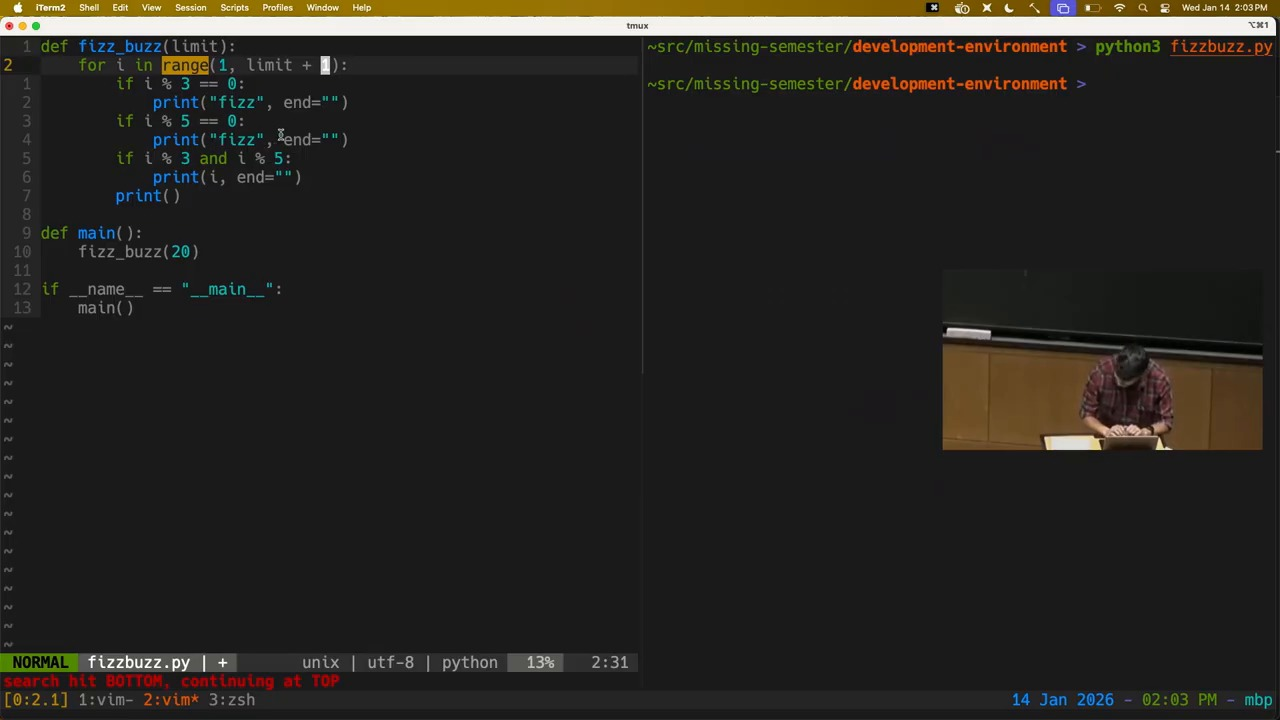
\includegraphics[width=0.92\textwidth]{figures/fig_15_fizz_line6.jpg}
\caption{打开行号后用 :6 跳到第 6 行，再用 ci" 把第二个 fizz 改成 buzz\vtag}
\end{figure}
\srcnote{00:27:30--00:27:45}
\end{minipage}


他发现程序对 3 和 5 的倍数都打印 fizz，于是要修改第二个。他用 \texttt{:6} 跳到第 6 行，并在左边打开了行号显示。光标在这一行的开头附近，按 \texttt{ci"}，即修改双引号内部：Vim 向前查找下一对双引号，删除里面的内容并进入插入模式。输入修改内容，按 Esc 回到普通模式。保存文件在 Vim 里是冒号进入命令模式，再按 \texttt{w} 写入文件；在别的 IDE 或工具里可能是别的键位。

\noindent\begin{minipage}{\textwidth}
\begin{figure}[H]
\centering
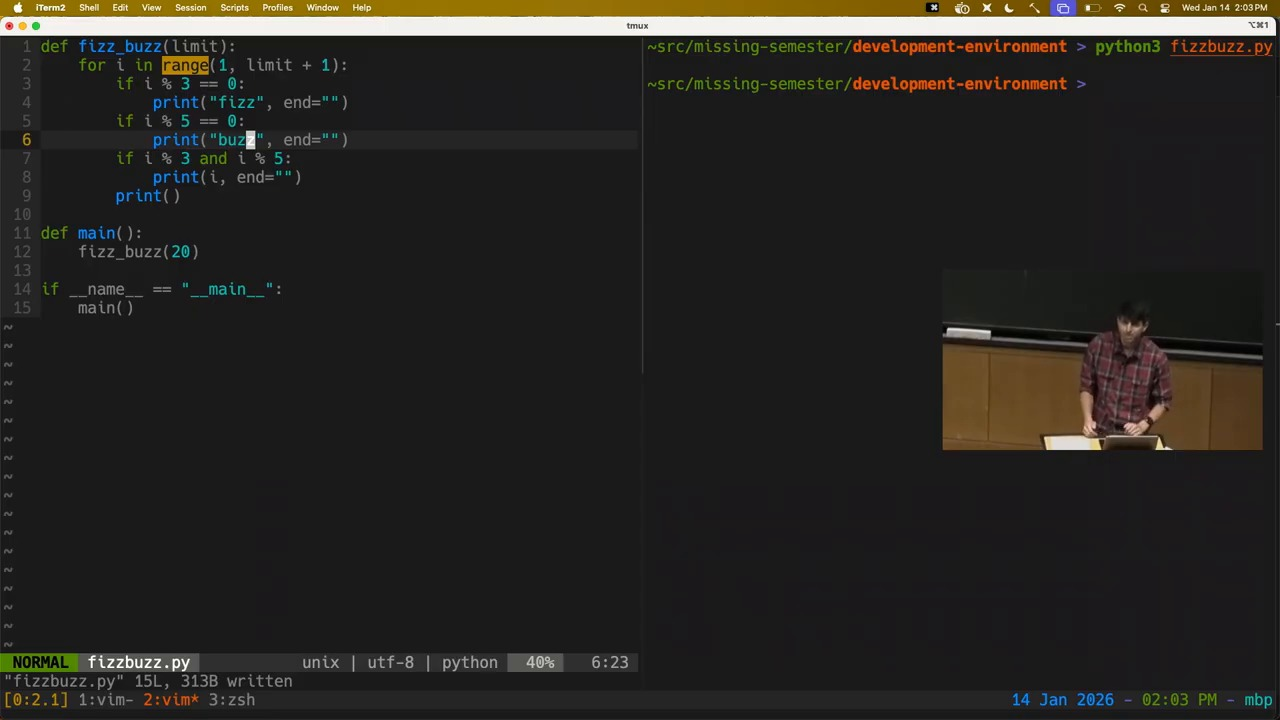
\includegraphics[width=0.92\textwidth]{figures/fig_16_fizz_done.jpg}
\caption{修复完成后的 FizzBuzz，保存并运行即可正确输出\vtag}
\end{figure}
\srcnote{00:28:15--00:28:30}
\end{minipage}


修好之后程序就能工作了。讲者说，今天讲义里的习题会给出一些指引，帮助大家真正建立使用这个强大软件的肌肉记忆。

\begin{warningbox}{演示代码的另一处问题}
讲义作者提醒：按讲义中的原始代码，第三个条件 \texttt{if i \% 3 and i \% 5:} 恰好在 \texttt{i} 既不是 3 的倍数也不是 5 的倍数时为真，是正确的；但 \texttt{range} 需要改成 \texttt{range(1, limit + 1)} 才能包含 \texttt{limit} 本身。这正是讲者用 \texttt{i} 插入 \texttt{1,}、再用 \texttt{a} 在末尾追加 \texttt{+ 1} 的原因。
\end{warningbox}

\subsection{本章小结}

Vim 的效率来自组合：移动作为名词，编辑命令作为动词，再加上计数和修饰符；绝大多数时间待在普通模式，只在需要输入时短暂进入插入模式。

\section{代码智能与语言服务器}

\subsection{语言服务器协议}

\noindent\begin{minipage}{\textwidth}
\begin{figure}[H]
\centering
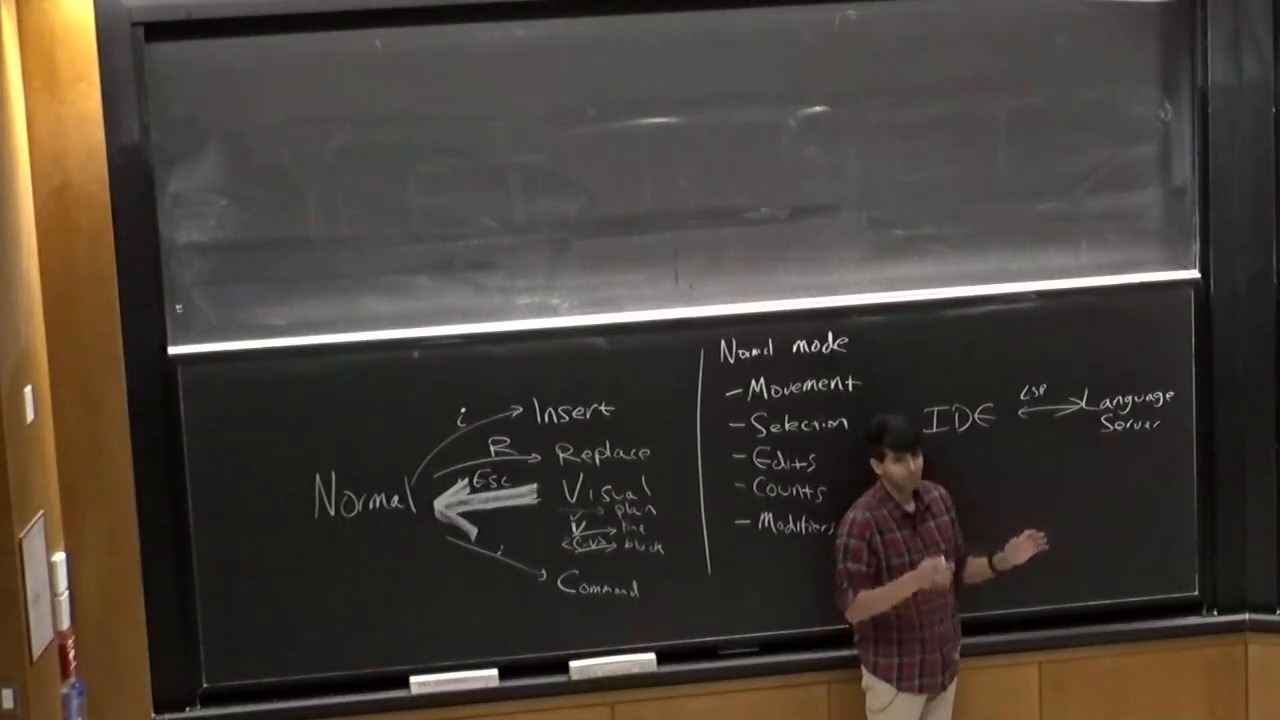
\includegraphics[width=0.92\textwidth]{figures/fig_17_lsp_board.jpg}
\caption{黑板上的示意：IDE 与语言服务器之间通过 LSP 通信\vtag}
\end{figure}
\srcnote{00:30:00--00:30:15}
\end{minipage}


讲者接下来讲更复杂的编辑器功能，特别是语言服务器。这部分他切换到 VS Code，因为那边配置得更全。IDE 通常提供许多针对特定编程语言的支持，比如自动格式化代码、边写边检查错误。但实现方式并不是 IDE 自己为每一种你可能用到的编程语言内置所有这些功能，而是有一个协议，让 IDE 与所谓的语言服务器（language server）通信，这个协议叫语言服务器协议（Language Server Protocol，LSP），由语言服务器提供特定语言的支持。

这样，一方可以构建 IDE、实现 LSP 协议的一侧；另一方实现协议另一侧的语言服务器；双方就能互通。讲者说，这把一个 $M \times N$ 的问题变成了 $M + N$ 的问题。所以如果用 IDE，就应该把它配置好，使它对你用的编程语言有完整的支持。讲义里有一些示例链接，一般也可以直接搜索，比如“怎样在 VS Code 里配置 Go 支持”。

\begin{importantbox}{为什么是 M+N}
假设有 $M$ 个编辑器、$N$ 种语言。没有共同协议时，每个编辑器都要为每种语言单独实现补全、跳转等功能，共 $M \times N$ 份实现；有了 LSP，每个编辑器只实现一次协议客户端，每种语言只实现一个语言服务器，总共 $M + N$ 份。
\end{importantbox}

\subsection{语言服务器能做什么}

为了说明值得花时间配置，讲者在一个随便找来的仓库里演示了语言服务器带来的功能。

\noindent\begin{minipage}{\textwidth}
\begin{figure}[H]
\centering
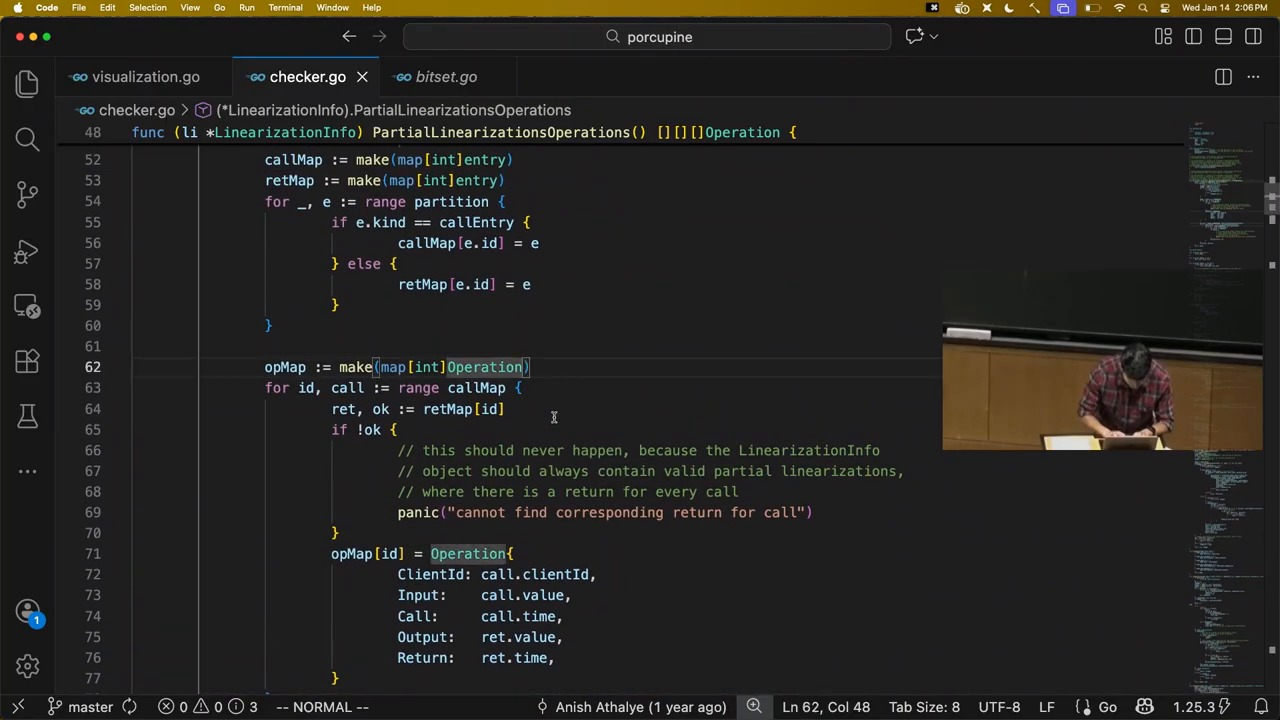
\includegraphics[width=0.92\textwidth]{figures/fig_18_completion.jpg}
\caption{在对象后输入点号，补全列表列出它的字段和方法\vtag}
\end{figure}
\srcnote{00:31:00--00:31:15}
\end{minipage}


首先是代码补全：在一个对象后面输入点号，就能看到它的所有字段和定义在它上面的方法，也就是行内代码补全，同时还有一定的文档。如果这些字段有文档字符串，就会直接在这里看到对应字段的说明。

\noindent\begin{minipage}{\textwidth}
\begin{figure}[H]
\centering
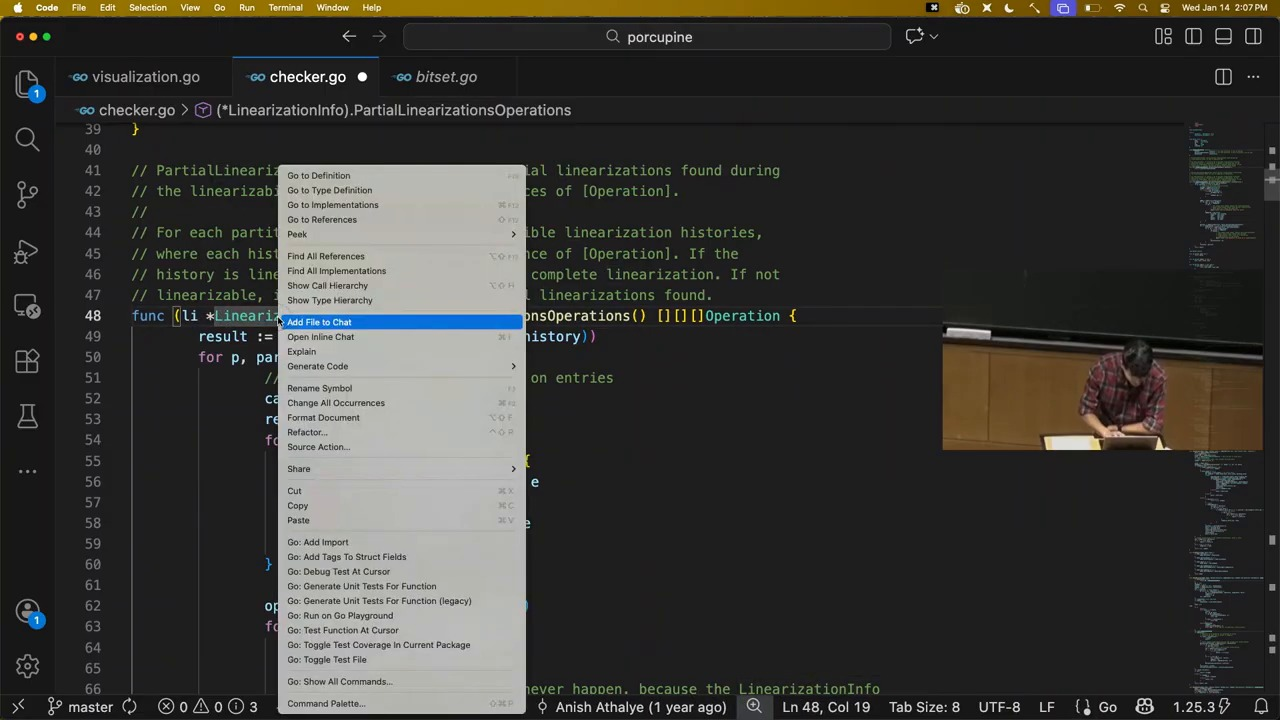
\includegraphics[width=0.92\textwidth]{figures/fig_19_goto_def.jpg}
\caption{右键菜单中的转到定义与查找所有引用\vtag}
\end{figure}
\srcnote{00:32:00--00:32:15}
\end{minipage}


另一个功能是跳转到定义：看代码时发现某个函数接受这个类型作为参数，可以右键点击它，选择“转到定义”，找到这个结构体的定义。讲者说这对四处跳转非常有帮助，否则你要怎样找到它定义在哪里？可能得在整个代码库里搜索、到处翻找。语言服务器对你的代码有语义上的理解，才能让 IDE 做到这一点。反过来也可以：定义了这个结构体之后，想知道哪里在用它，可以查找它的所有引用。

\noindent\begin{minipage}{\textwidth}
\begin{figure}[H]
\centering
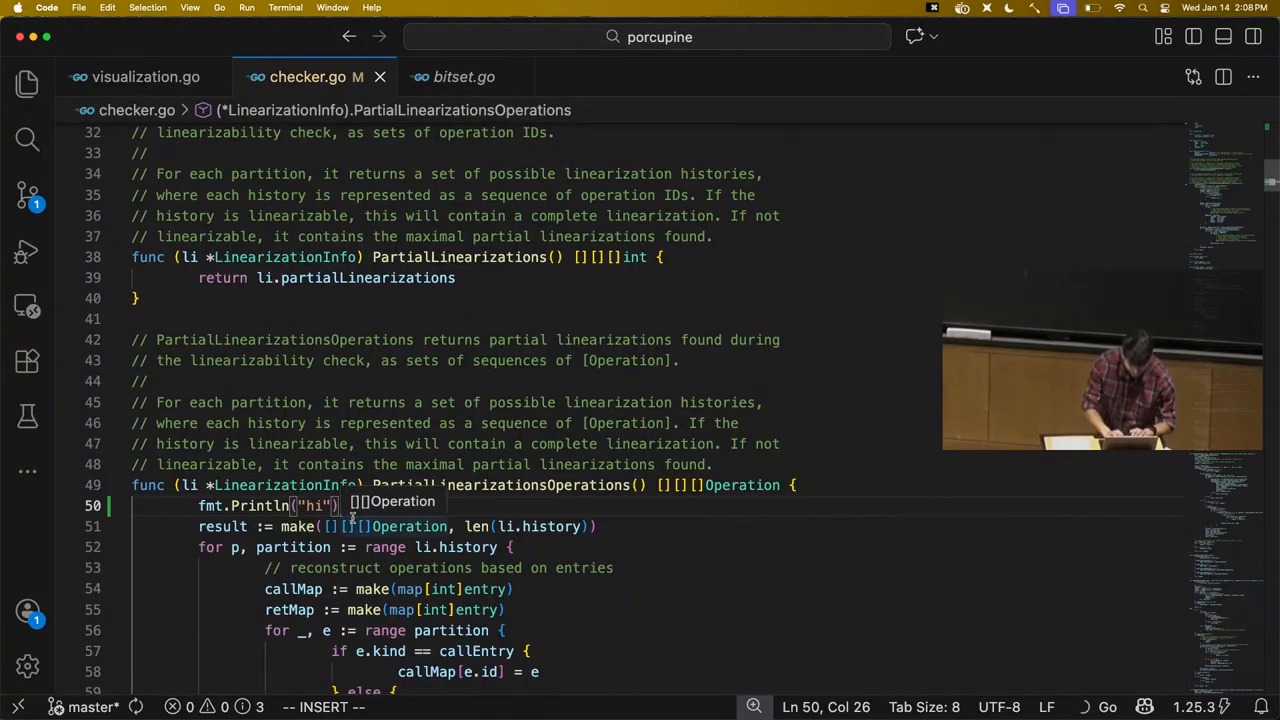
\includegraphics[width=0.92\textwidth]{figures/fig_20_imports.jpg}
\caption{保存时语言服务器自动补上缺失的 fmt 导入\vtag}
\end{figure}
\srcnote{00:33:00--00:33:15}
\end{minipage}


还有一大堆改善体验的功能，比如帮你管理导入：如果使用某个模块却没有导入，比如用 \texttt{fmt.Println}，会看到红色波浪线，提示找不到这个模块；但保存时，语言服务器会判断出你在用 \texttt{fmt.} 什么东西，大概是想导入 \texttt{fmt}，于是替你加上了导入语句。还有各种代码质量检查：调用了不存在的方法，IDE 里会直接显示“这个类型没有这个名字的方法”。这样你能边写边发现错误，而不是等到编译或运行测试时。

\begin{practicebox}{配置你的语言支持}
讲义作者整理：为你最常用的语言安装语言服务器（例如 Python 的 Pyright 或 basedpyright、Go 的 gopls、Rust 的 rust-analyzer），然后在编辑器中验证以下功能都能工作：补全、悬停文档、转到定义、查找引用、重命名符号、保存时格式化和实时错误提示。
\end{practicebox}

\section{AI 辅助开发}

\subsection{三种形态}

讲者说，在某种程度上这是最难准备的主题，因为他不确定大家在使用这些工具方面的背景。所以先做个小调查：谁用过专门为写代码设计的 AI 工具，比如 AI 自动补全、行内聊天或编码智能体，不算单独使用 ChatGPT 之类的 LLM。只有大约 20\% 的人举手，于是他决定多讲基础，讲义里还有很多进阶内容。

背景是：自 2021 年年中 GitHub Copilot 推出以来，LLM 在帮人写代码方面越来越好，现在这些工具非常流行。人们用这些模型写代码主要有三种方式：自动补全，与前面看到的自动补全字段或方法名形式相同，但强大得多；行内聊天；以及编码智能体。

\subsection{AI 自动补全}

\noindent\begin{minipage}{\textwidth}
\begin{figure}[H]
\centering
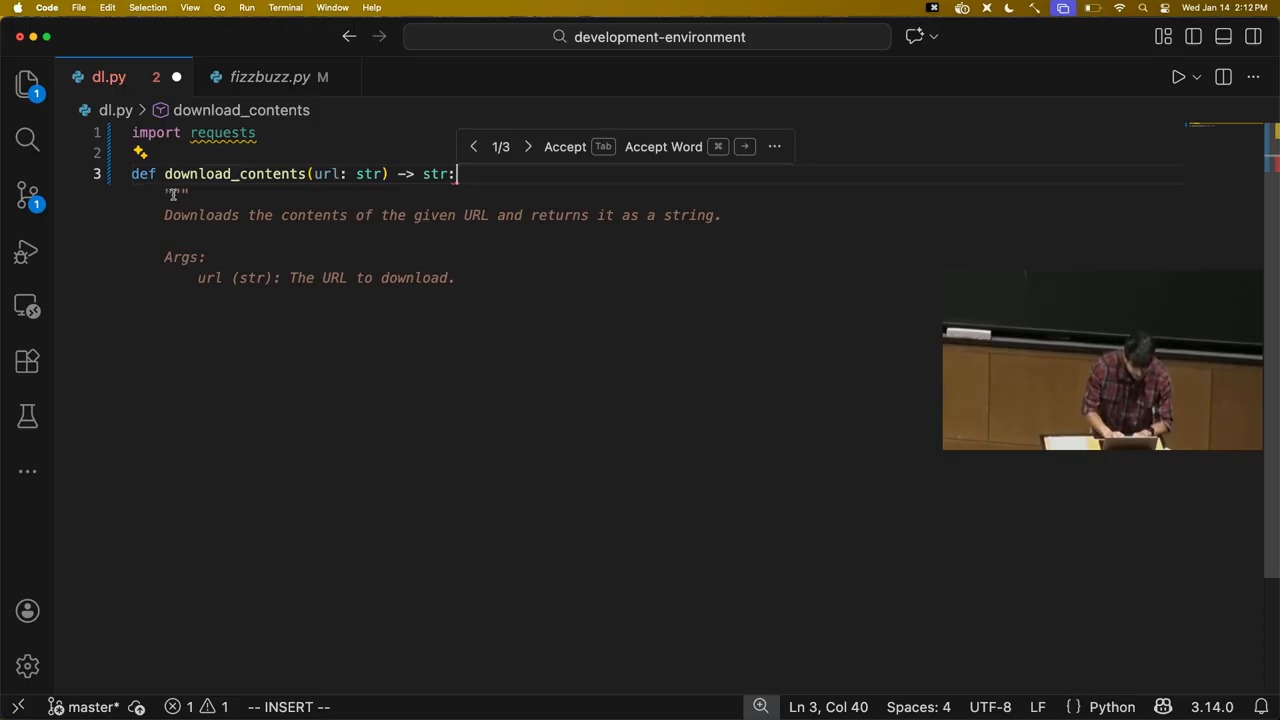
\includegraphics[width=0.92\textwidth]{figures/fig_21_autocomplete.jpg}
\caption{只写了函数签名，Copilot 就以灰色文字建议出整个函数体\vtag}
\end{figure}
\srcnote{00:37:15--00:37:30}
\end{minipage}


如果使用集成了 AI 的 IDE，比如带 GitHub Copilot 的 VS Code、Cursor，或者现在市面上上百种软件中的任何一种，就会有非常聪明的自动补全。讲者以写一个脚本为例：下载这份讲义的内容并提取其中的所有链接。我们也许完全有能力自己从头写，但 AI 可以加快速度。比如用 Python 写，先导入一个做 HTTP 请求的库，立刻就看到了自动补全：AI 建议“你导入了 HTTP 库，也许想写一个下载文件的函数”。他没有采纳，而是自己输入：函数叫 \texttt{download\_contents}，接受一个字符串 URL，返回一个字符串。

有同学问他用的是什么扩展。讲者说这次演示用的是 VS Code 加 GitHub Copilot，讲义里有推荐软件的章节；但粗略地说，课程不想强烈推荐某个软件或教某个软件的用法，更关注底层概念，这些在各种工具之间是共通的，比如在 Cursor 里做同样的事，效果完全一样。

可以看到，开始写代码后，AI 模型会补全到光标之后，以稍微灰色的文字显示建议的代码片段，甚至可以在几个候选补全之间切换：可以从 LLM 采样多个结果，看看它认为可能怎样补全，按 Tab 接受。这个例子里他只写了函数签名，AI 就写出了整个函数体，省了很多输入。

\begin{warningbox}{接受补全前一定要读}
讲者提醒：这些模型只是概率模型，在大量数据上训练，再加上一些别的技巧，它们并不具备人类那样的智能。所以接受 AI 补全时，一定要看一遍，确认它在做你想要的事；有时它不对，你需要修改它的输出，或者干脆自己从头写。
\end{warningbox}

\subsection{用注释和文档字符串引导}

\noindent\begin{minipage}{\textwidth}
\begin{figure}[H]
\centering
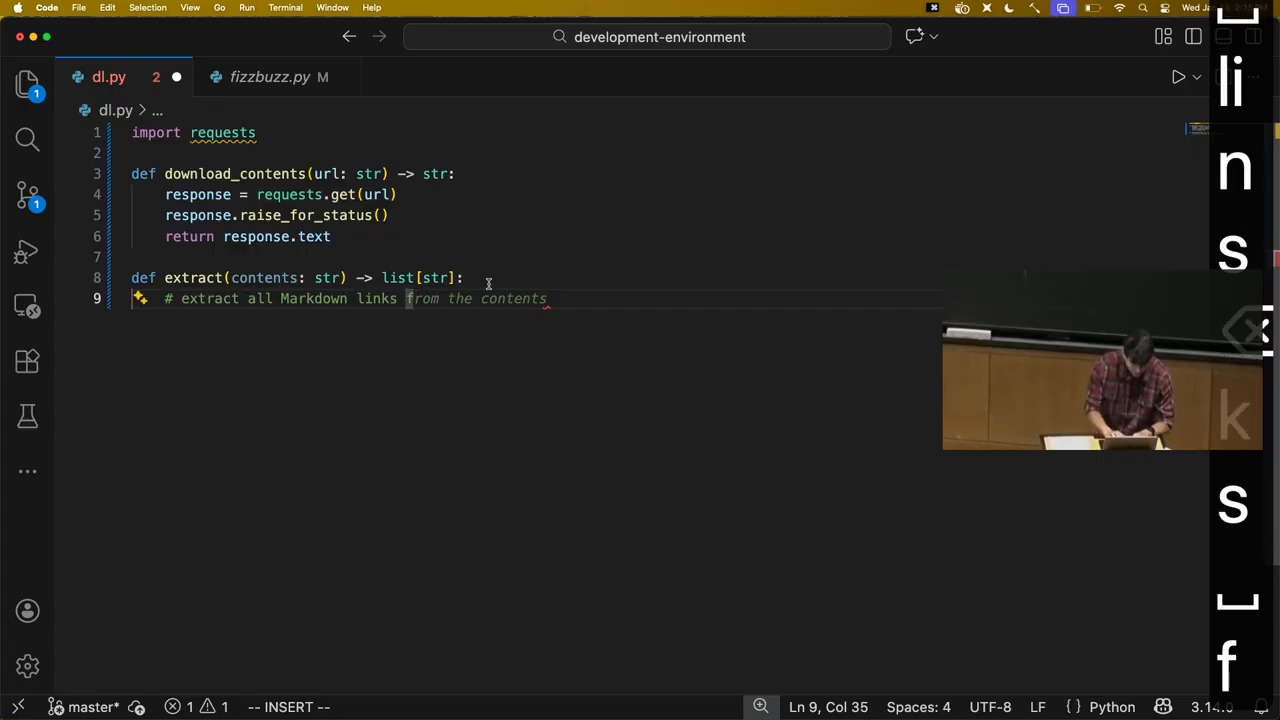
\includegraphics[width=0.92\textwidth]{figures/fig_22_comment_steer.jpg}
\caption{写下一行注释说明要提取 Markdown 链接后，补全才开始导入 re 并写出正则\vtag}
\end{figure}
\srcnote{00:39:30--00:39:45}
\end{minipage}


标准用法是被动的：它一直在运行，你写着代码，它随时冒出来说“我可以这样补全”，看起来不错就按 Tab 接受。另一种用法是用注释引导它。讲者继续写脚本：定义一个函数 \texttt{extract}，接受内容，返回字符串列表。AI 很乐意补全，但它是根据目前写的程序来补全的，并不知道他想提取链接，最可能的补全只是把内容按行切分，对他想写的东西毫无用处。

引导的一种方式是写注释。他写下“从内容中提取 Markdown 链接”，AI 甚至会补全这条注释。接受之后，它开始建议真正与任务相关的东西。有时它不会一次补全整个函数体，而是部分补全，可以一段段按 Tab 接受：导入正则表达式库，定义一个正则模式，写完函数，看起来都正确。

有同学问什么时候写注释、什么时候用侧边的聊天框。讲者说那个聊天框是“用智能体构建”，等讲编码智能体时会讲这种交互方式。但总的来说，这种自动补全只补全光标之后的代码，所以只能做范围很窄的修改。比如这里它在函数中间导入了一个库，很凌乱，他并不想这样，但 Tab 补全只能补全光标之后的内容；如果想修改文件其他部分，这种交互方式就不合适。

\noindent\begin{minipage}{\textwidth}
\begin{figure}[H]
\centering
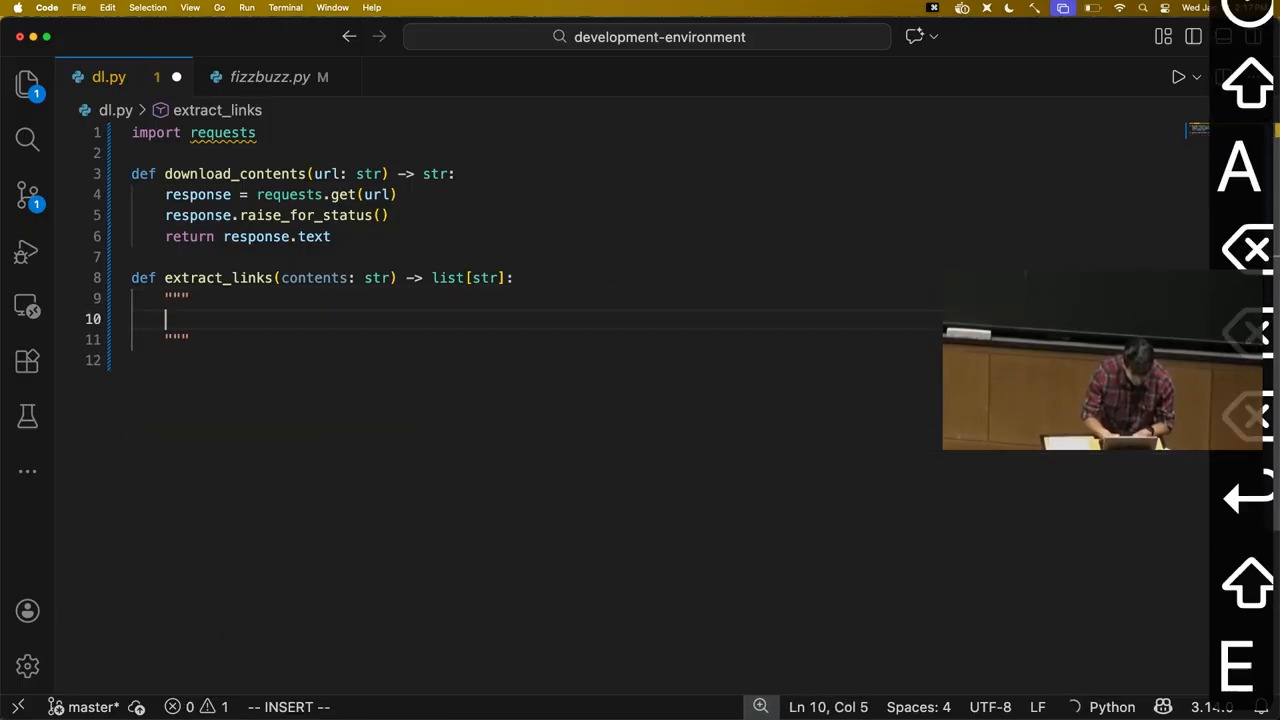
\includegraphics[width=0.92\textwidth]{figures/fig_23_docstring.jpg}
\caption{把函数命名为 extract\_links 并写好文档字符串后，补全一次写出整个实现\vtag}
\end{figure}
\srcnote{00:41:30--00:41:45}
\end{minipage}


讲者说，这里只是演示可以用代码注释引导 AI，实践中你可能不会这样做，而是写得更有描述性：把函数命名为 \texttt{extract\_links}，再用文档字符串引导，写上“从给定的 Markdown 文档中提取所有链接”，说明参数是内容、返回提取出的链接列表。这样 AI 会以同样的方式补全，而且一次写完整个实现。这是好得多的写法，因为文档字符串对将来真正有用，而前面那种注释没什么用。用 AI 自动补全写代码时，常见做法是写一些小注释引导 AI，比如用注释勾勒出函数的大纲，让 AI 在注释下方 Tab 补全，然后把注释删掉，因为它们在最终产物里没多大用处。

\subsection{行内聊天}

\noindent\begin{minipage}{\textwidth}
\begin{figure}[H]
\centering
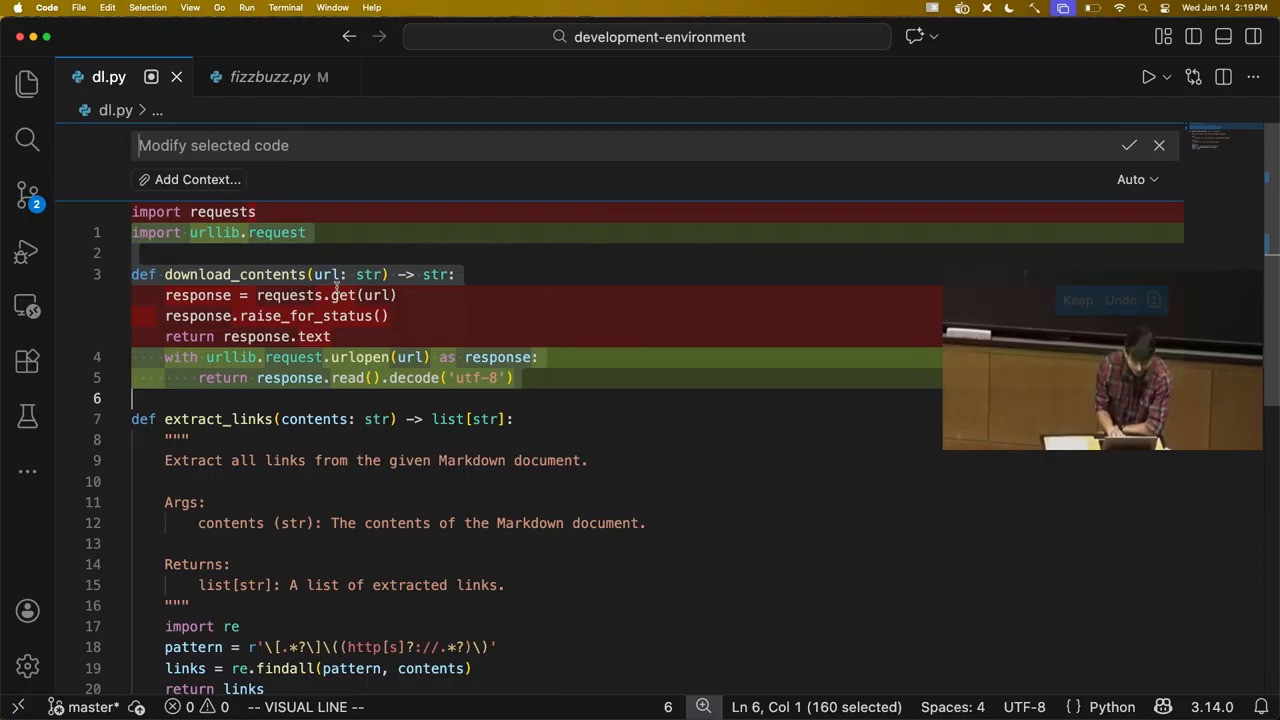
\includegraphics[width=0.92\textwidth]{figures/fig_24_inline_chat.jpg}
\caption{选中使用第三方库的代码块后用 Cmd+I 要求不用第三方库，AI 以红绿差异给出修改\vtag}
\end{figure}
\srcnote{00:43:30--00:43:45}
\end{minipage}


另一种交互方式叫行内聊天（inline chat）：选择一个光标位置、一行或一段文本，然后直接给 AI 输入，引导它以某种方式修改。假设代码里用了一个第三方库，而希望这个脚本没有外部依赖。讲者回到前面的 Vim 部分：他在 VS Code 里开启了 Vim 键位，于是按 Shift+V 进入可视行模式，再按几次 \texttt{j} 选中这一段。在带 GitHub Copilot 的 VS Code 里，按 Ctrl+I 或 Cmd+I 调出行内聊天。选中文本后就可以朝特定方向引导 AI，他输入“不要使用第三方库”并回车。

AI 对代码提出了一系列修改，以差异的形式显示，红色和绿色分别是删除和添加的内容。它修改了已有的代码，这和补全光标之后的内容已经不同了：这里是在编辑已经存在的东西。他检查了这些修改，看起来都合理，就保留了 AI 建议的修改。

\noindent\begin{minipage}{\textwidth}
\begin{figure}[H]
\centering
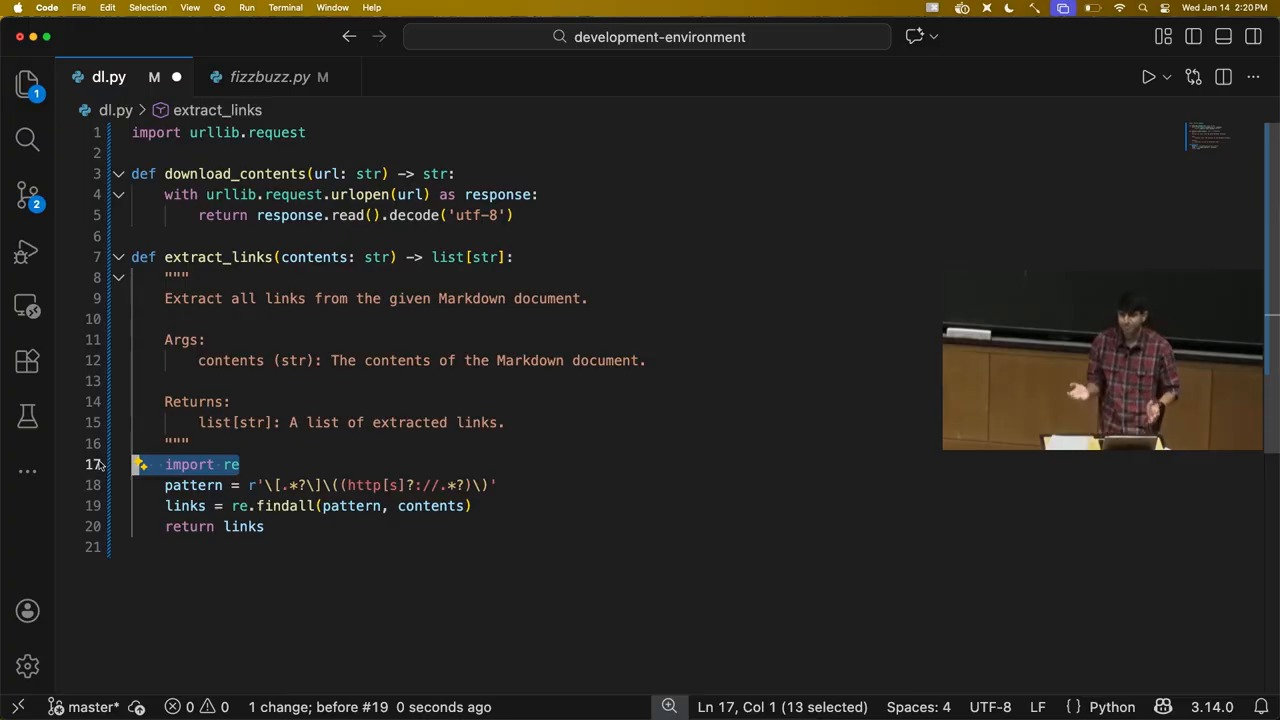
\includegraphics[width=0.92\textwidth]{figures/fig_25_inline_limit.jpg}
\caption{只给出一个光标位置要求移出 import 时，这个实现只能修改选区内的代码\vtag}
\end{figure}
\srcnote{00:45:00--00:45:15}
\end{minipage}


有同学问：如果完成请求需要的不只是选中的部分呢？讲者说这取决于具体实现，并现场演示：把光标放在这里，要求“把这个 import 移到外面”。结果没有做出有用的事，因为这个实现只修改他给出的选区内的内容。他说这是一个很新、很开放的领域，其他编辑器的行内聊天可以修改其他位置；但它的设计仍然是“这里有一块东西，按某种方式修改它”。具体取决于你使用的工具。

\subsection{答疑}

有同学问这样使用 AI 是否需要网络连接。讲者说大多数情况下需要：这些工具使用的模型非常大，要在复杂的硬件上才能以合理的性能做推理，有些是万亿参数的模型，需要巨大的内存和高端 GPU。也有更小、能力更弱、能在笔记本上运行的本地模型，但效果不如大模型；它们仍然要做大量计算，所以会比较快地耗电。

讲者说时间不够了，只讲完了今天计划内容的一小部分，于是做了个小投票：大家是否有兴趣在之后的课上深入讲编码智能体？相当一部分人举手，所以他们会考虑调整课程安排，把剩下的内容推迟到之后的课。讲义作者注：从课程表看，第七讲正是“智能体编程”。

关于隐私，有同学问能否在使用这些 AI 工具时防止代码被上传到云端。讲者说可以，但有个星号：有些工具可以在设置里打开一些默认关闭的选项，声明你需要额外的隐私，比如服务商不保留你的代码和你发送的提示词。但你是在信任他们这样做，目前基本没有常用的技术手段来保证隐私；这方面有一些研究，但还不普及。如果真的要隐私，就需要在本地运行模型。

有同学问：Python 很灵活，可以在函数中间导入模块，Tab 补全在不那么灵活的语言里会不会效果更差？讲者说按他的经验仍然不错。还有一个没来得及演示的功能：有些补全模型还会预测光标位置，猜测你接下来想把光标移到哪里。比如它意识到你要用正则库，在填写函数实现之前，补全建议会先让光标跳到顶部，下一个建议是 \texttt{import re}，再下一个是跳回来填写函数体。

\begin{importantbox}{在合适的抽象层次上使用 AI}
讲者说，这些模型和工具在不断改进、不断引入新能力，你要不断更新对 AI 工具能力的直觉。一个好的工作方式是处在合适的抽象层次上：很简单的事 AI 能轻松搞定，你不必花时间写；但如果交给它对当前 AI 来说太难的任务，它会以各种方式出错，写出看起来大致正确却有 bug 的代码，或者陷入混乱、做出疯狂的事。而今天完全做不到的事，三个月后可能就能轻松完成。所以要持续使用、持续试探它们的边界。
\end{importantbox}

有同学问能否让 AI 解释为什么这样写代码，或者在生成之前先向你提问、告诉你它有多确信。讲者说在目前讲到的交互方式里不行，但在编码智能体里可以，它们更像对话工具，大致像接入了你代码的 ChatGPT，你可以直接和它交谈，让它向你提问，也可以问它问题。但要记住它们是概率性的下一个词预测器：有时说的话看似合理且正确，有时乍看合理却完全错误。所以使用这些工具的方式和把任务委派给员工不一样，讲者笑说，希望员工不会像这些 AI 模型那样“PUA”你。

最后有同学问 VS Code 有没有推荐的 AI 扩展。讲者说听众大多是 MIT 学生，所以推荐 GitHub Copilot，因为它免费：注册 GitHub 教育版（GitHub for Education）就能免费使用，需要验证你是学生或教师；而很多其他工具要每月付 20 美元左右。粗略地说，这些工具的能力相差不大，尤其是在入门阶段。

\begin{knowledgebox}{课上没讲到的部分}
讲义作者补充：课程讲义中这一讲还包括编码智能体的用法、正则表达式以及编辑器中的查找替换。正则表达式在第一讲的 \texttt{grep}、\texttt{sed} 中已经出现过，在 Vim 中可以用 \texttt{/\{regex\}} 搜索、用 \texttt{:s/旧/新/g} 在当前行替换、用 \texttt{:\%s/旧/新/g} 在整个文件中替换。编码智能体则在第七讲专门讲解。
\end{knowledgebox}

\section{总结}

\begin{itemize}
\item 开发环境可以是 tmux 加终端编辑器，也可以是 VS Code 这样的图形化 IDE，各有适用场景。
\item Vim 是模式编辑器，普通模式是默认位置；它的界面像一门编程语言，移动、选择、编辑、计数、修饰符可以自由组合。
\item Vim 键位在 VS Code、Emacs、bash、zsh 乃至 Claude Code 中都可用，学会一次处处受益。
\item 语言服务器协议把编辑器与语言支持解耦，提供补全、转到定义、查找引用、自动导入和实时错误检查。
\item AI 自动补全只补全光标之后的内容，可用注释或文档字符串引导；行内聊天能修改选区内已有的代码；更复杂的任务交给编码智能体。
\item AI 的输出必须审查；在合适的抽象层次上使用它，并随着工具进步不断更新直觉。
\end{itemize}

\begin{practicebox}{自测}
\begin{enumerate}
\item 用 Vim 命令描述：删除到行尾；修改当前单词；把光标移到下一个逗号；删除三行。
\item \texttt{ci"} 与 \texttt{da"} 有什么区别？
\item 为什么用 \texttt{a} 比 \texttt{l} 加 \texttt{i} 更好？
\item LSP 解决了什么问题？为什么说它把 $M \times N$ 变成了 $M + N$？
\item 举一个 AI 自动补全不适合、而行内聊天更适合的例子。
\end{enumerate}
\end{practicebox}

\end{document}
